%%%%%%%
% Ch4 %
%%%%%%%

\chapter{Ponts universels}
	\begin{wrapfigure}[5]{l}{6 cm}
	\vspace{-5mm}
	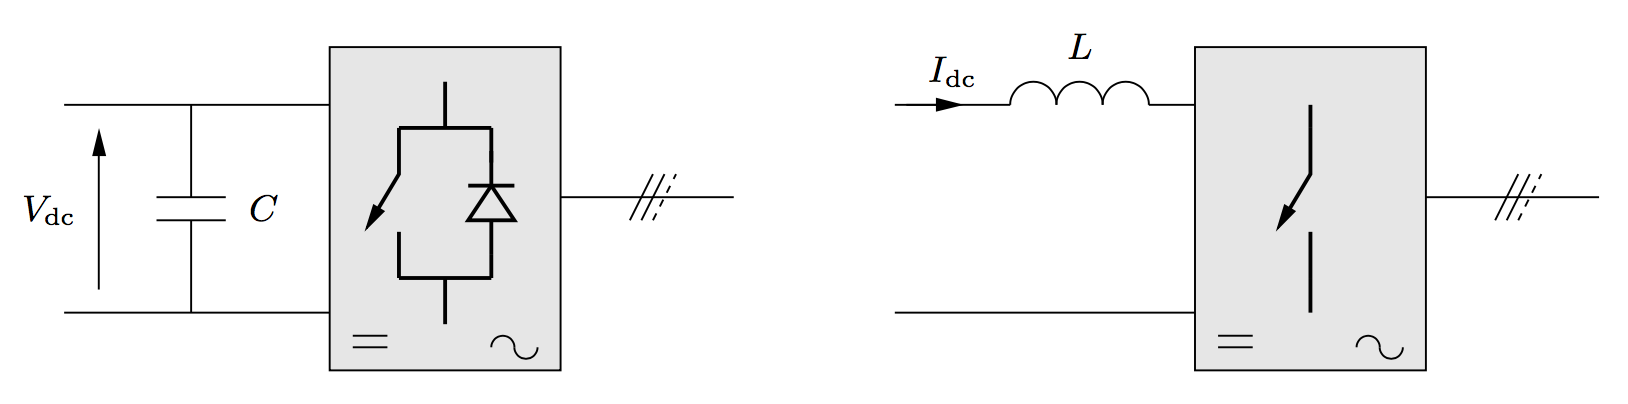
\includegraphics[scale=0.2]{ch4/1}
	\captionof{figure}{}
	\end{wrapfigure}
	Les \textbf{onduleurs autonomes} possèdent généralement une structure en pont et sont constitués d'intérupteurs commandables. Ils peuvent être alimenté par une source de tension continue (voltage source converter, VSC) ou par une source de courant continue (CSC), les deux modèles diffèrent par un condensateur ou une inductance dans le bus d'entrée. Ils peuvent fonctionner en \textbf{redresseur}. Les hacheurs \textbf{multi-quadrants} utilisé entre autre pour la commande de moteur à courant continu ont la même topologie avec une commande semblable. 
	
	\begin{minipage}{0.5\textwidth}
		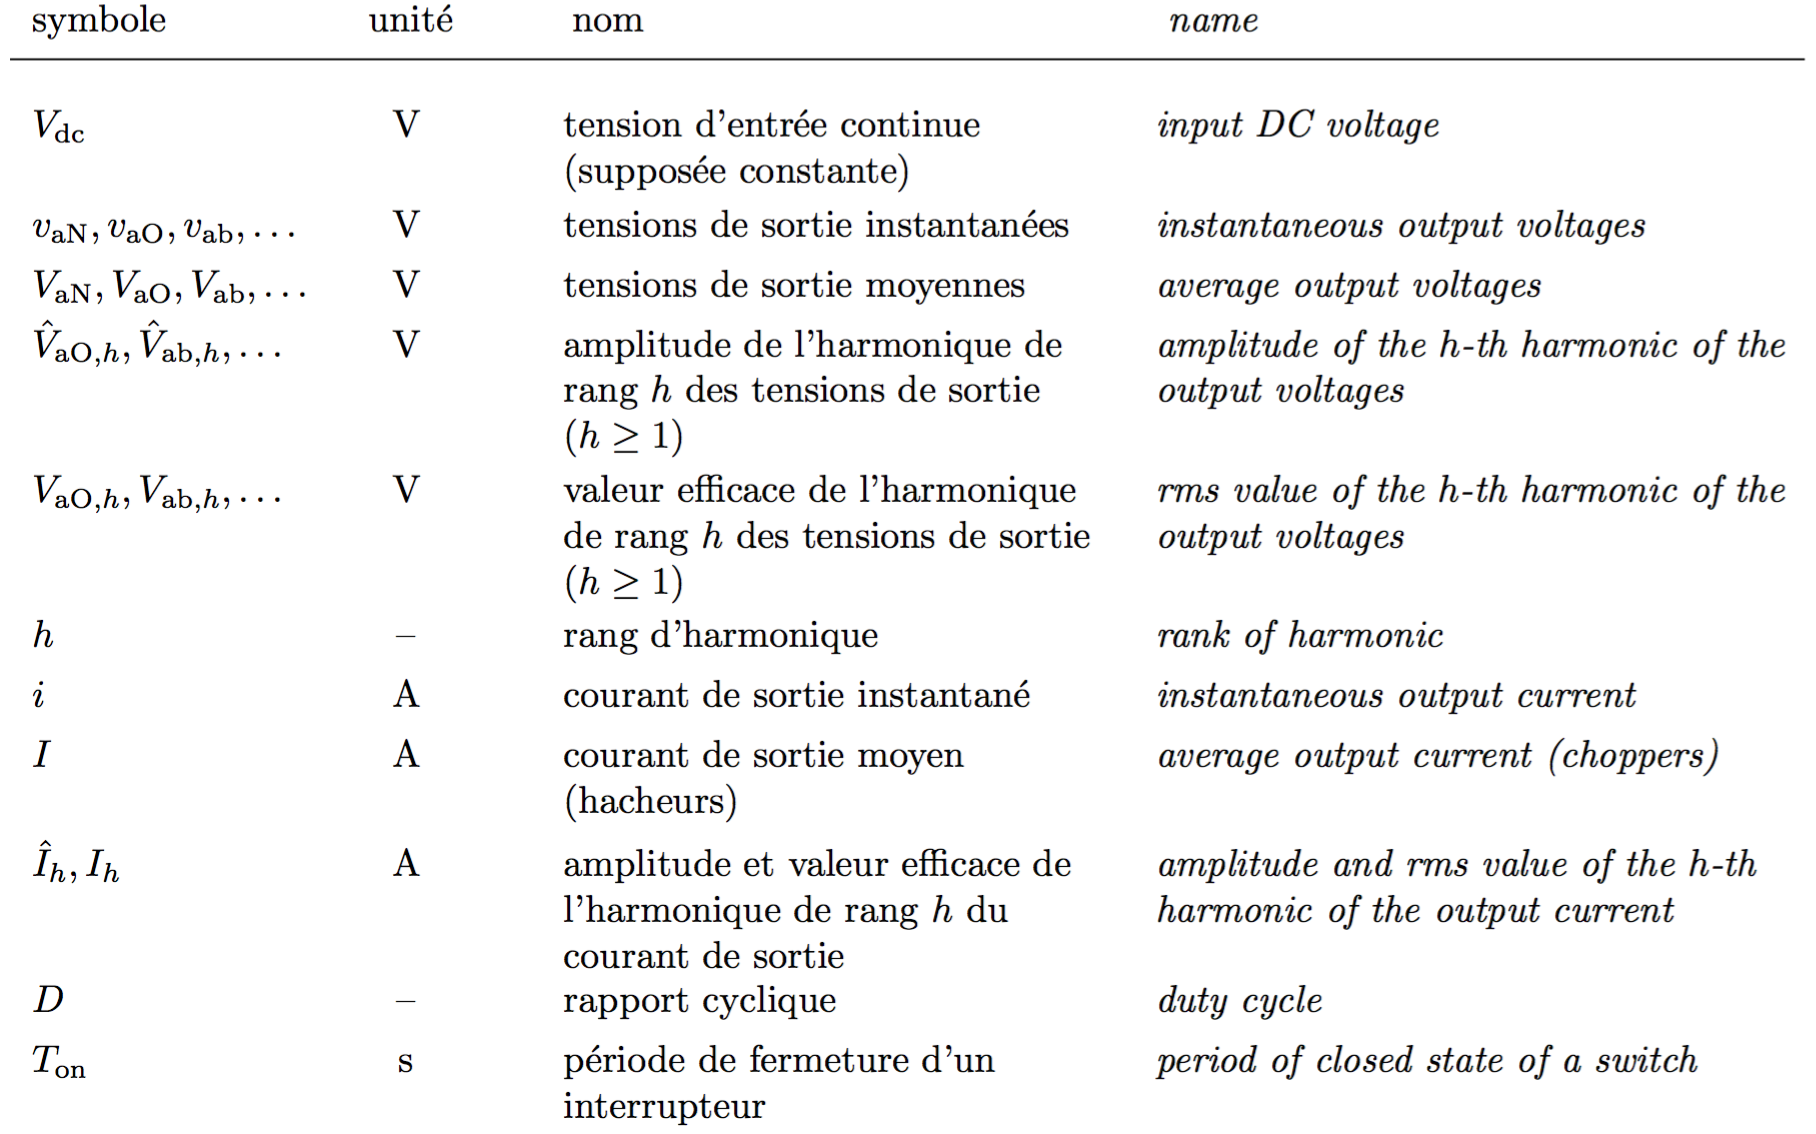
\includegraphics[scale=0.25]{ch4/2}
	\end{minipage}
	\begin{minipage}{0.5\textwidth}
		\vspace{3mm}
		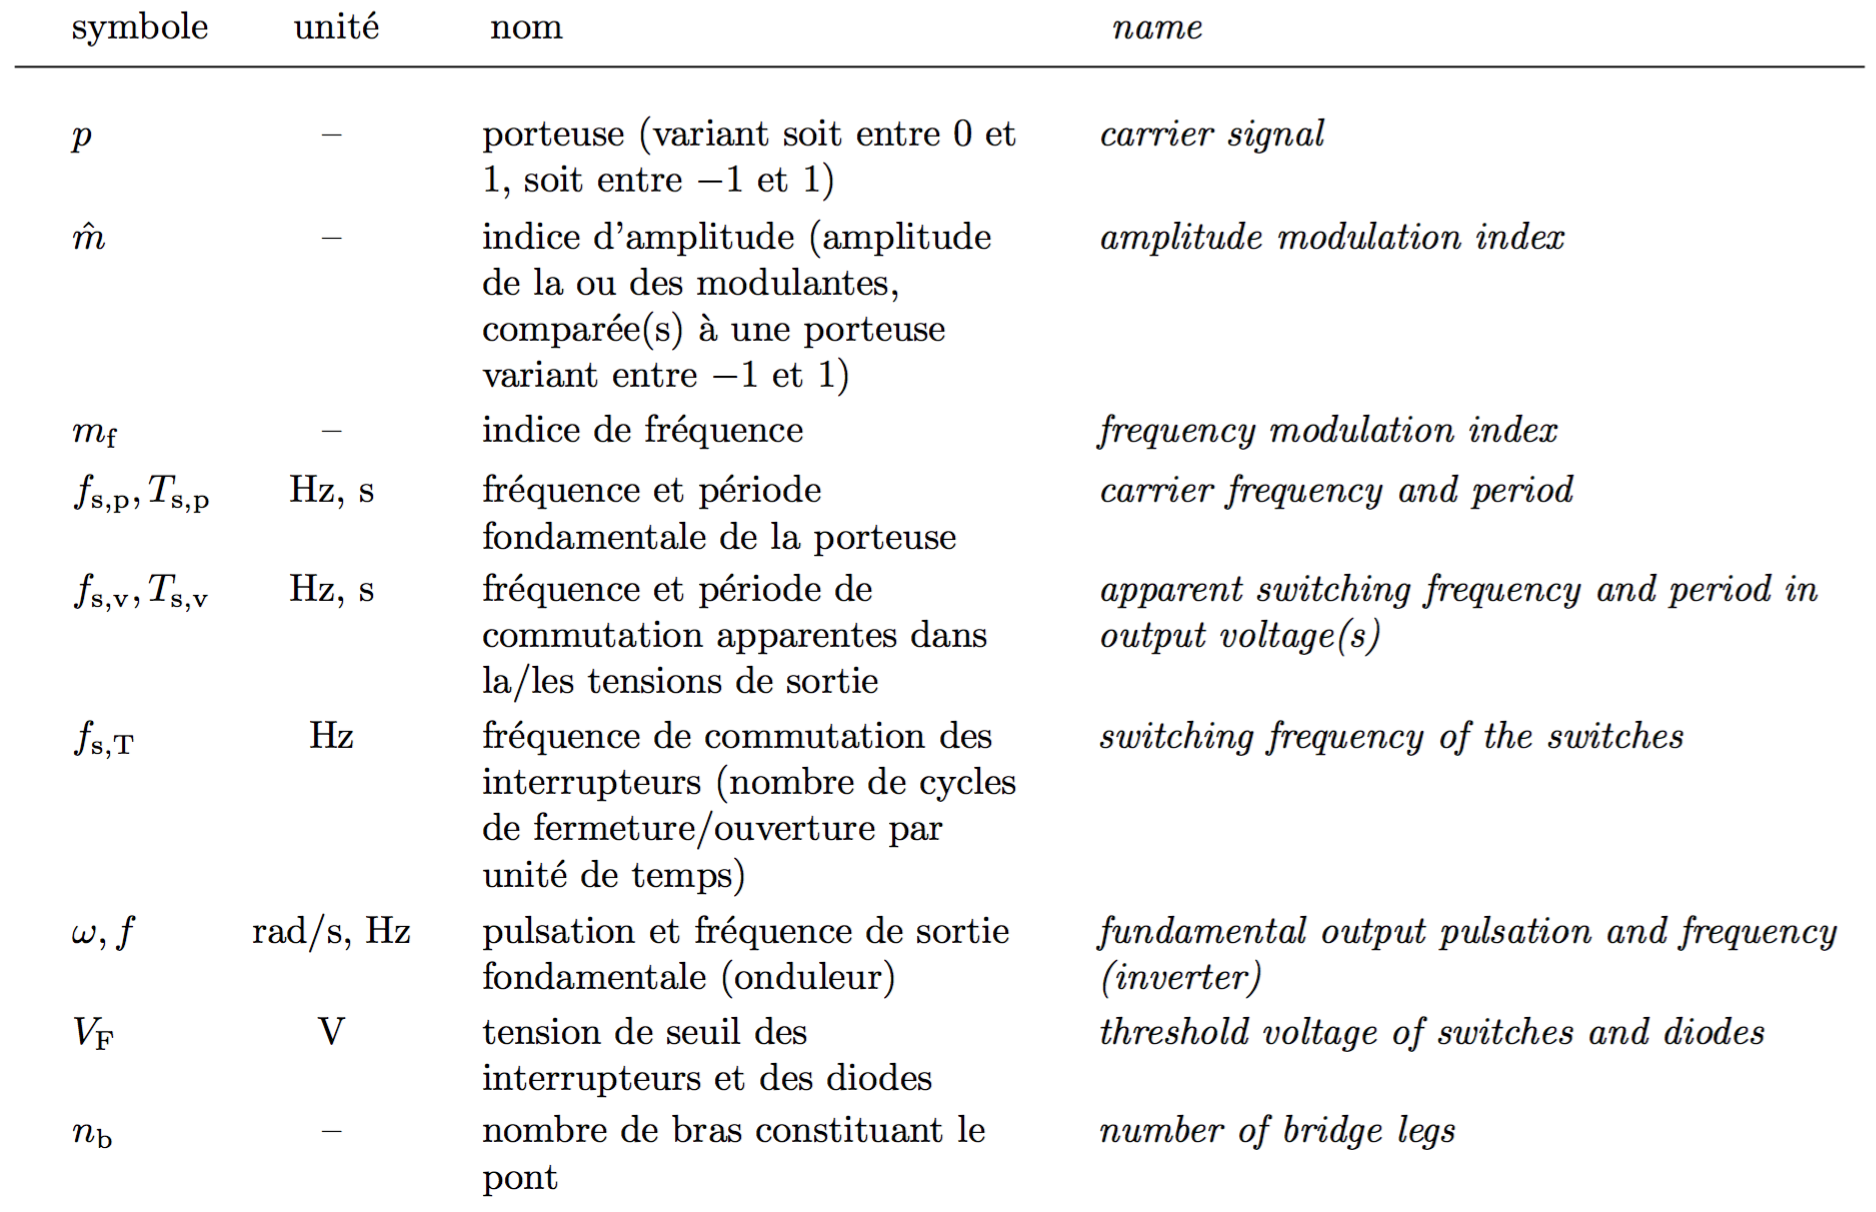
\includegraphics[scale=0.25]{ch4/3}	
	\end{minipage}
	\captionof{table}{Liste des abréviations et symboles.}
	
\section{Caractéristiques des interrupteurs commandables}
	\begin{wrapfigure}[4]{r}{5 cm}
	\vspace{-5mm}
	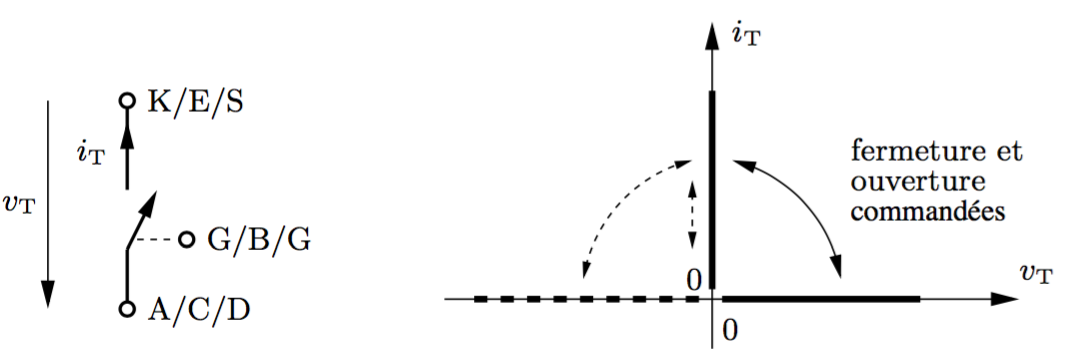
\includegraphics[scale=0.25]{ch4/4}
	\captionof{figure}{}
	\end{wrapfigure}
	Ci-contre, la caractéristique tension-courant idéalisée d'un interrupteur commandable. Le 2${ème}$ quadrant ne nous intéresse pas puisque la tension $v_T$ y est négative et est exclue lorsqu'une diode est raccordé en anti-parallèle sur l'interrupteur. \\
	
	\begin{wrapfigure}[6]{l}{6 cm}
	\vspace{-5mm}
	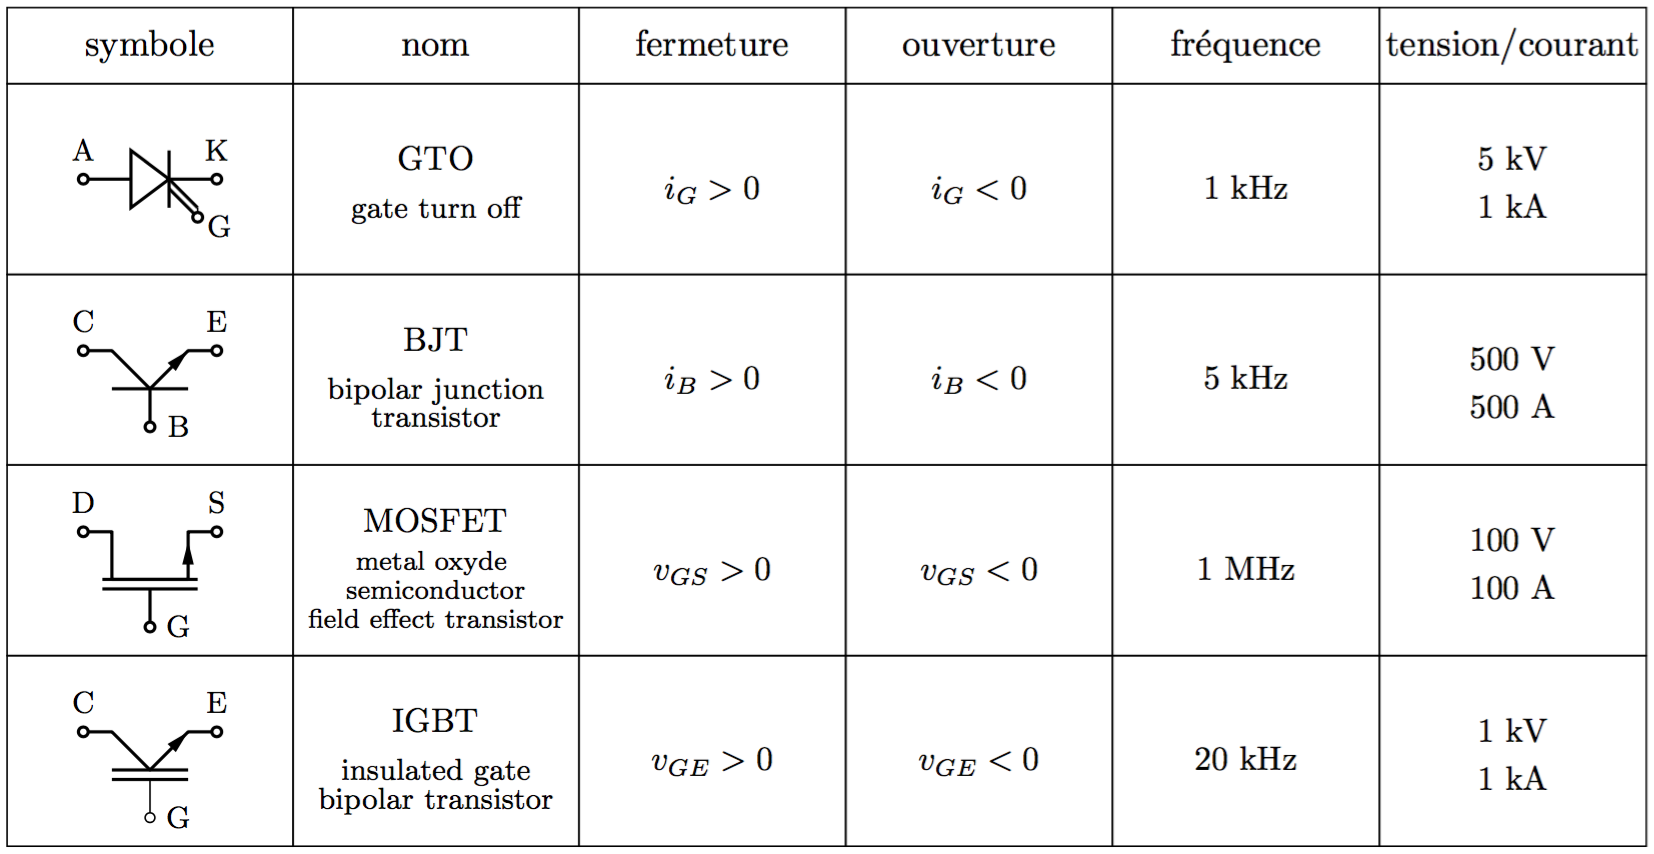
\includegraphics[scale=0.2]{ch4/5}
	\captionof{figure}{}
	\end{wrapfigure}
	Ils sont tous \textbf{unidirectionnnels} donc le courant ne peut circuler que de l'anode A vers la cathode K, du collecteur C vers l'émetteur E ou du drain D vers la source S. L'\textbf{électrode de commande} (gachette G, base B ou grille G) permet d'effectuer la fermeture et ouverture de l'interrupteur grâce à une tension ou un courant. 
	
	La tension $V_{T,max}$ et le courant $I_{T,max}$ maximum supportée ou conduit par l'interrupteur sont limités. On peut faire des montages en série ou parallèle pour augmenter la puissance nominale mais il va falloir faire une répartition uniforme du courant et tension. La commutation entre l'état passant et bloqué prend un certain temps plus ou moins important, ce qui limite la fréquence de commutation $f_{s,T}$. Durant ces intervalles, la tension et le courant sont tout deux importants et donnent lieu à des \textbf{pertes de commutation}.
	
\section{Convertisseurs à source de tension : généralités}
	\subsection{Topologie et réalisation pratique}	
		\begin{wrapfigure}[12]{l}{7cm}
		\vspace{-5mm}
		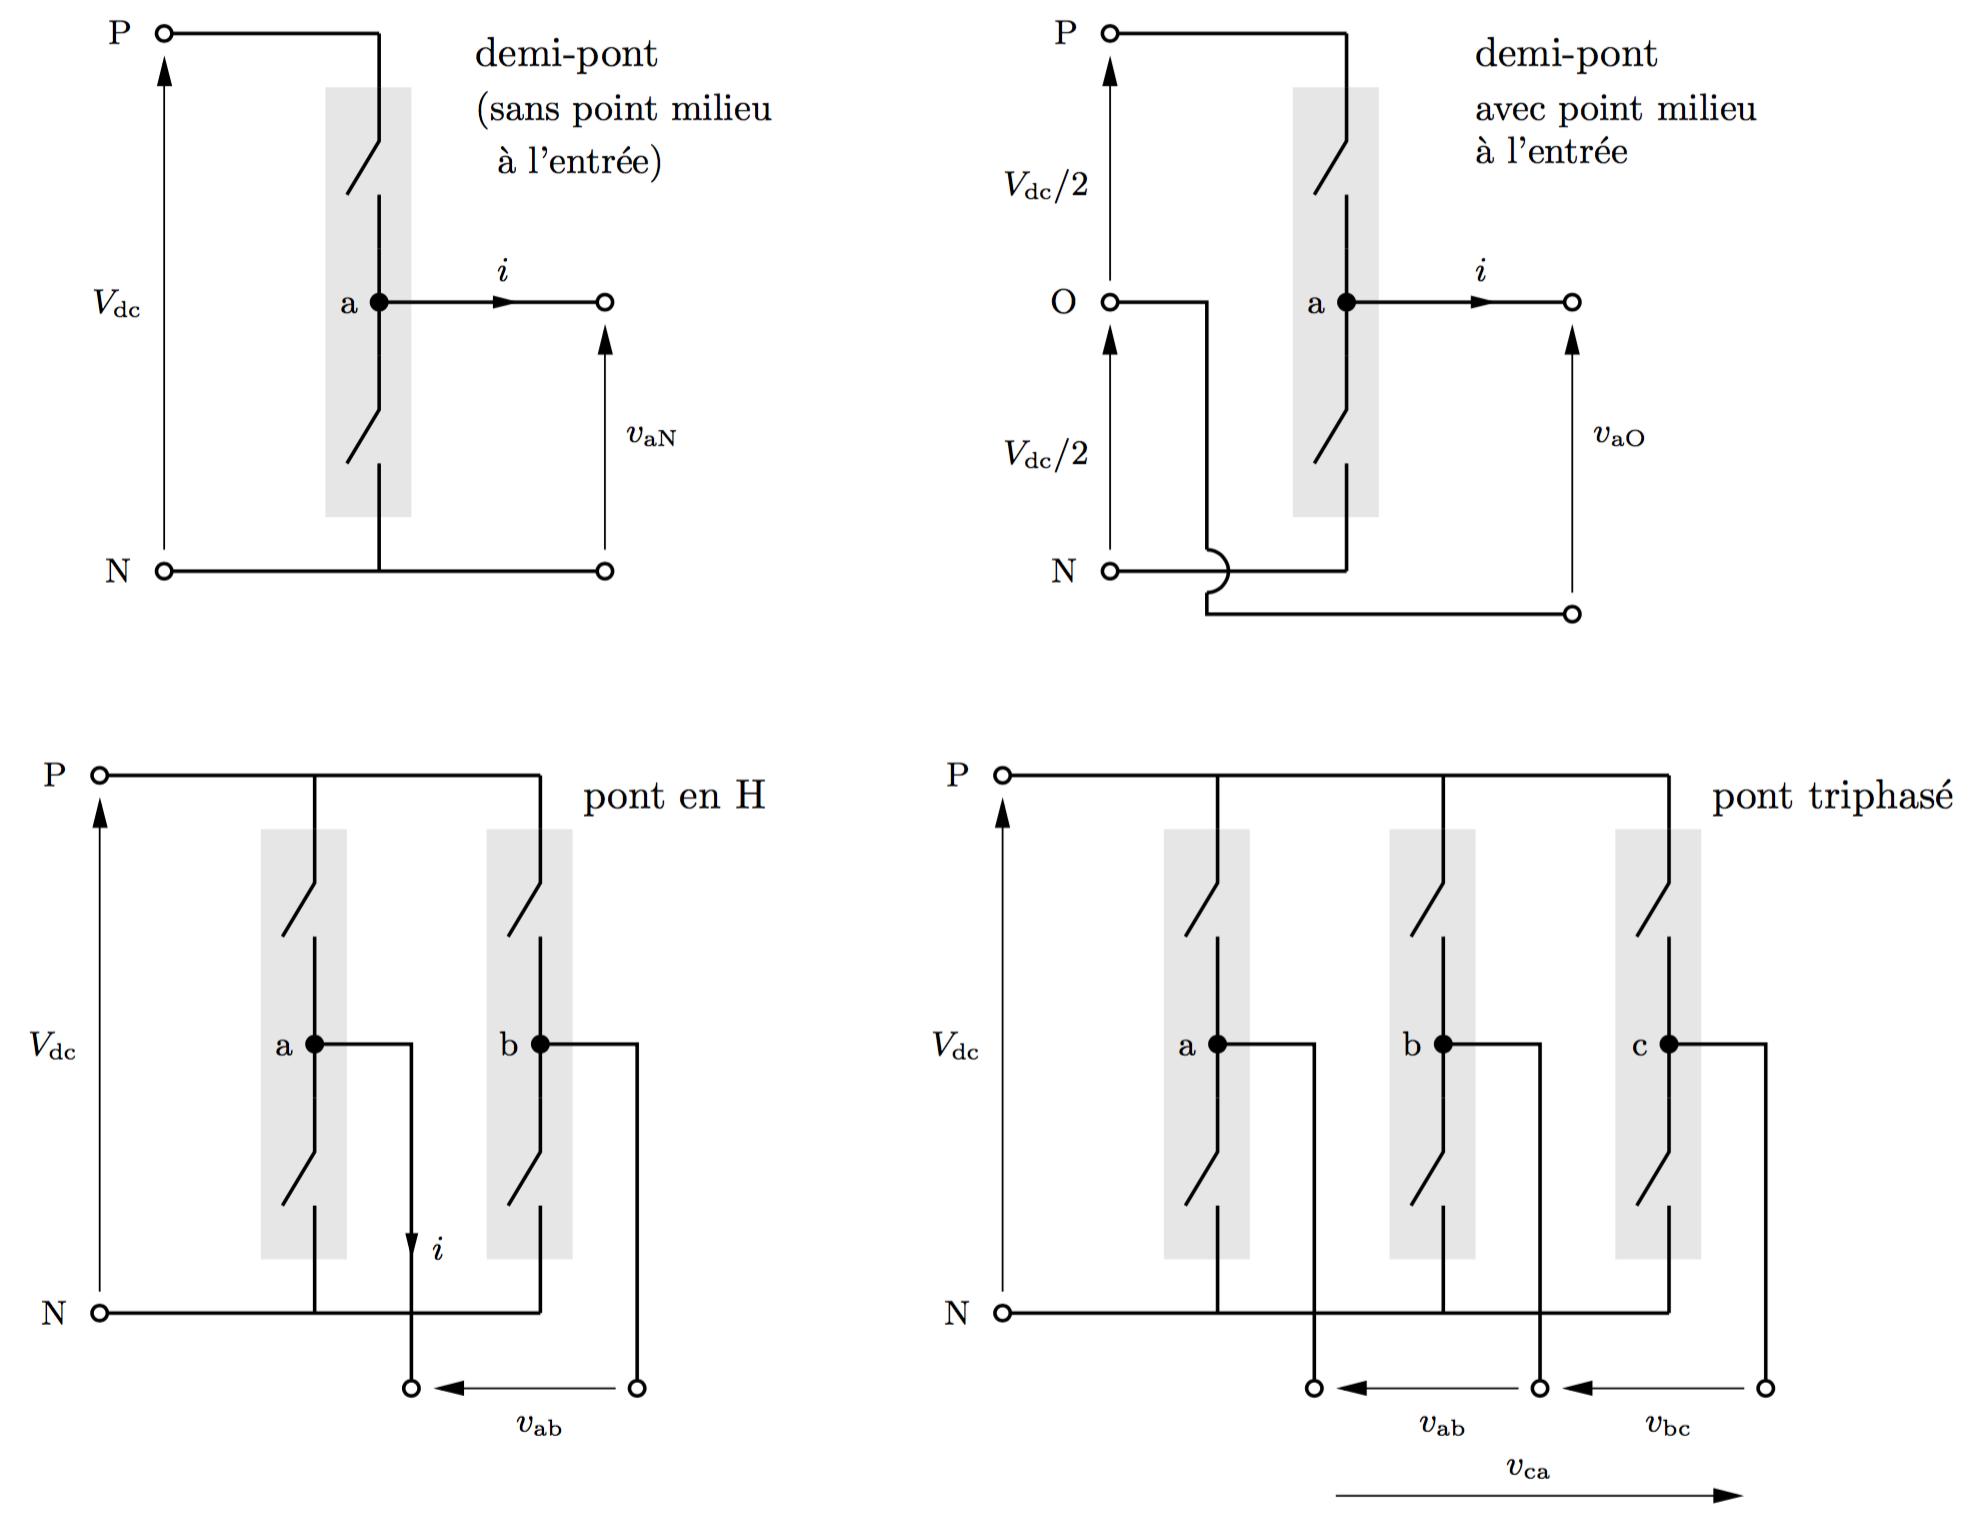
\includegraphics[scale=0.2]{ch4/7}
		\captionof{figure}{}
		\end{wrapfigure}
		La figure ci-contre reprend 4 topologies de ponts à 1,2 ou 3 bras. Chaque bras comprend un interrupteur bidirectionnels en courant et commandables et est relié entre les pôles N et P de l'entrée. Les points milieux a, b et c constituent les bornes de sortie, ainsi que N et O dans le demi-pont. Pour éviter un court-circuit, les 2 interrupteurs d'un même bras de peuvent être fermés en même temps, sous risque de détruire les interrupteurs. En jouant avec les interrupteurs on forme des tensions de sortie différentes. \\
		
		Pour le premier demi-pont, on a $v_{aN} = 0$ ou $v_{aN} = V_{dc}$. Dans le second, $v_{aN} = \pm V_{dc}/2$. Pour les deux derniers, $v_{aN} = 0$ ou $v_{aN} = \pm V_{dc}$. On peut donc fabriquer une ou des tensions continues ou alternatives de valeur moyenne désirée.  
		
		\begin{wrapfigure}[9]{r}{4cm}
		\vspace{-5mm}
		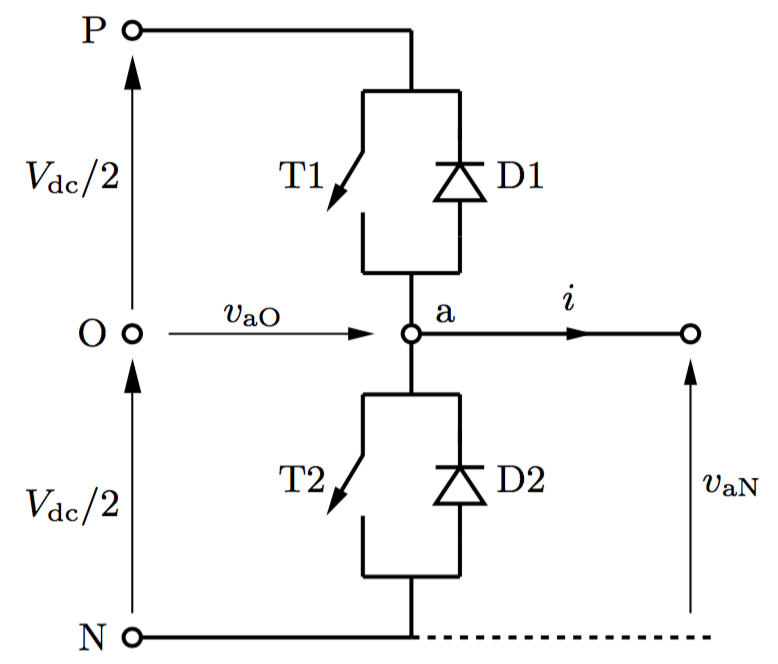
\includegraphics[scale=0.3]{ch4/8}
		\captionof{figure}{}
		\end{wrapfigure}
		\ \\ Ci-contre on peut voir que chaque bras est constitué de 2 interrupteurs commandables et unidirectionnels en courant (GTO, BJT, IGBT, MOSFET, ...), T1 et T2 et de 2 diodes de roue libre, D1 et D2 en  anti-parallèle sur les interrupteurs. Pour éviter le court-circuit via les 2 diodes, il faut impérativement que la tension d'entrée soit \textbf{positive}. Si T1 est fermé, T2 doit être ouvert, a est alors relié à P et D2 est polarisé en inverse. Si $i>0$, il circulera dans T1 sinon dans D1. Pareil si T2 est fermé, T1 est ouvert et a est raccordé à N, D1 est polarisé en inverse. Si $i>0$ il passera dans D2, sinon dans T2. \\
		
		Interessons nous à $v_{aO}(t)$ du demi-pont en supposant $V_{dc}<0$ et cst. $v_{aO}(t)$ ne dépend que de l'état des interrupteurs, si T1 est fermé, $v_{aO(t)} = + V_{dc}/2$ et si T2 est fermé $v_{aO}(t) = -V_{dc}/2$ quel que soit le signe du courant. On peut donc, en jouant sur l'intervalle de fermeture des T obtenir une consigne moyenne entre $+V_{dc}/2$ et $-V_{dc}/2$. \\
		
		Vu la vitesse de commutation, il faut intercaller un petit interval de temps ou les 2 T sont ouverts en même temps pour éviter le court-circuit. On parle de temps mort (dead time) $t_{\Delta}$. Durant $t_{\Delta}$, c'est le signe du courant qui détermine $v_{aO}$. 
		
	\subsection{Conduction dans les composants semi-conducteurs et pertes associées}
		\begin{wrapfigure}[8]{l}{5.5cm}
		\vspace{-5mm}
		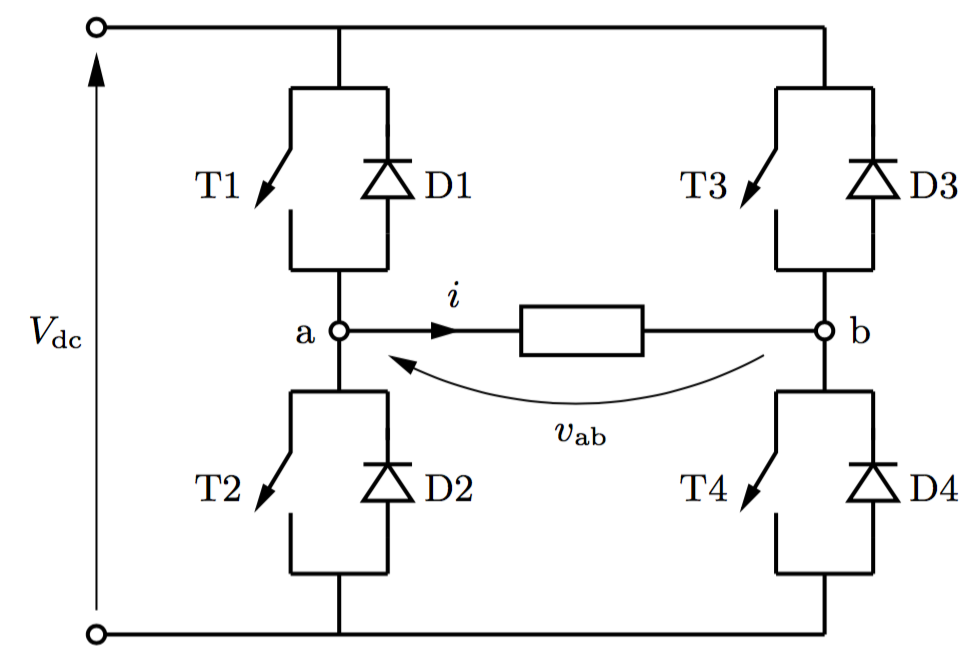
\includegraphics[scale=0.3]{ch4/9}
		\captionof{figure}{}
		\end{wrapfigure}
		Lorsque les interrupteurs conduisent, il y a la \textbf{tension résiduelle} faible mais non nulle à leur bornes (1 à 3V), donnant lieu aux pertes de conduction. En état ouvert, le courant de fuite sont négligeables. Selon les états ouverts et fermé, 2 fois neufs combinaisons existent (4 $\times$ états complémentaires, 4 $\times$ un bras sans fermeture et l'état tous ouverts). Pour exemple, si la conduction se fait au travers D2 et D3 dans un pont en H, il vient :
		\begin{equation}
			V_{ab} = -V_{dc}-V_{F,D2}-V_{F,D3}-(R_{on,D2}+R_{on,D3})i,
		\end{equation}
		où les pertes de conduction instantannées (en W) s'obtiennent en multipliant la seconde partie par $i$. A courant négatif, à conduction dans T2 et T3 on a :
		\begin{equation}
			V_{ab} = -V_{dc}+V_{F,T2}+V_{F,T3}-(R_{on,T2}+R_{on,T3})i. 
		\end{equation}
		
	\subsection{Commutation dans un bras et pertes associées}
		\begin{wrapfigure}[8]{r}{8cm}
		\vspace{-5mm}
		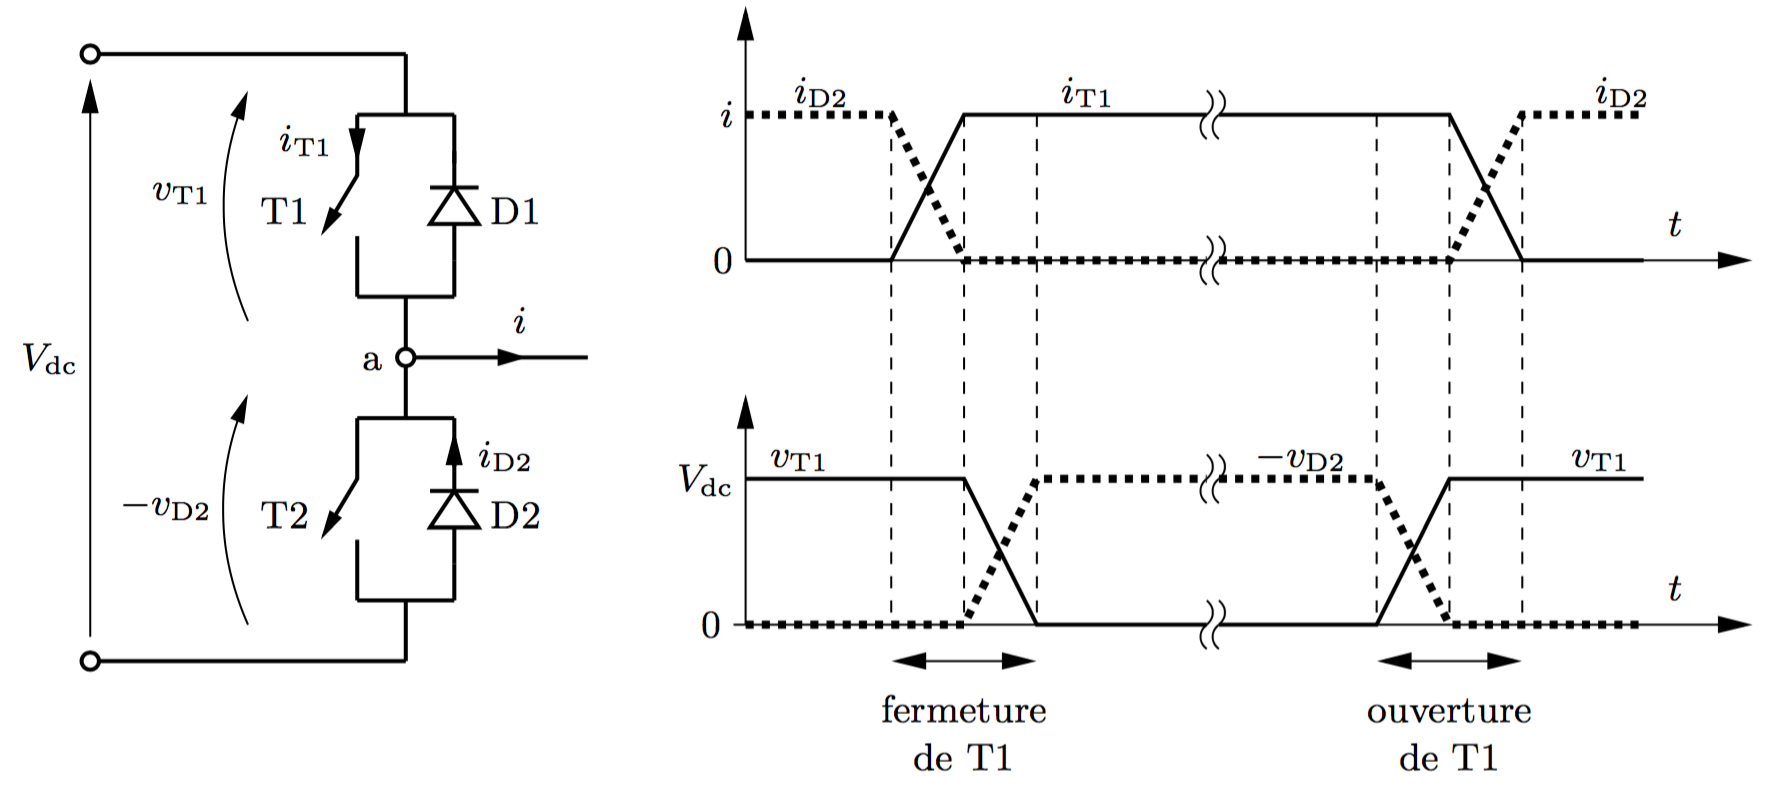
\includegraphics[scale=0.25]{ch4/10}
		\captionof{figure}{}
		\end{wrapfigure}
		Considérons un demi-pont dont le point milieu est connecté à une charge inductive, le courant ne pouvant varier que lentement et circule entièrement soit dans T1 soit D2 ou les 2 durant la commutation : 
		\begin{equation}
			i = i_{T1}+ i_{D2}.
		\end{equation}		 
		Du côté de la tension :
		\begin{equation}
			V_{dc} = v_{T1} - v_{D2},
		\end{equation}
		où $v_{T1}$ et $v_{D2}$ sont pratiquement nulle en conduction et égal à $V_{dc}$ et $-V_{dc}$ en non-conduction et varient entre les 2 valeurs en commutation. Les formes d'onde nous indique que, lorsque la fermeture de T1 est commandé, $i_{T1}$ croît à partir de 0 alors que D2 continue à conduire avec $v_{D2} = 0$ et $v_{T1} = V_{dc}$. Ce n'est que lorsque D2 s'arrête de conduire que $-v_{D2}$ peut monter jusque $V_{dc}$ et $v_{T1}$ chuter jusque 0. Pour son ouverture, il faut $v_{T1}$ monte jusque $V_{dc}$ pour que D2 se retrouve polarisé en direct et puisse conduire. \\
		
		Durant la commutation, $p_{T1} = v_{T1}i_{T1}$ est non négligeable et l'intégrale sur un intervalle de commutation donne une énergie d'autant plus grand que $V_{dc}, i$ et les temps de commutations sont grands. On en vient à introduire alors la fréquence de commutation. Sur base des données dans les datasheets, les pertes de commutation dans les bras (en W) peuvent être approchées comme :
		\begin{equation}
			P_{com} = f_{s,T} (E_{on,ref}+ E_{off,ref})\frac{V_{dc}}{V_{dc,ref}}\frac{i}{i_{ref}},
		\end{equation}
		où les E sont les énergies susmentionnées relatives aux valeurs de référence.
	
\section{Hacheurs - modulation de largeur d'impulsions (MLI)}
	 \textbf{Pulse width modulation (PWM)} est une des méthode de commande des bras du convertisseur. La fréquence de commutation est maintenue constante et pour chaque bras, la période de commutation est scindée en 2 partie où c'est d'abord l'interrupteur supérieur qui est fermé puis l'inférieur. En modulant la durée des sous-intervalles, on génère la tension moyenne. \\
	 
	 Les tensions sont entachés d'une série d'harmoniques en raison de la commutation. Les charges inductives font que les courants sont en meilleur état. Notons qu'en cas de commande à hystérésis, la fréquence de commutation n'est pas constante et les harmoniques sont alors de fréquence variable (problème du filtre). \\
	 La \textbf{MLI intersective} consiste à déterminer les instants de commutation pour un bras en comparant la \textbf{porteuse p(t)}, signal triangulaire de fréquence $f_{s,p}$ et la \textbf{modulante}, image de la tension souhaitée. Pour les ponts en H dans le cas monophasé, il est possible d'utiliser la même modulante pour les 2 bras (modulation bipolaire) ou d'en prendre 2 séparés (modulation unipolaire) avec la même porteuse. Pour un pont onduleur/redresseur \textbf{triphasé} il faut considérer trois modulantes formant un système triphasé équilibré. \\
	 
	 Lorsque la commande est faite avec de l'électronique analogique, la comparaison de p(t) et m(t) est fait telle quelle. Avec de l'électronique digitale, même résultat obtenu sans réelle comparaison (rapport cyclique). 
	 
	 \subsection{Demi-pont}
	 	\subsubsection{Sans point milieu à l'entrée}
	 		\begin{wrapfigure}[8]{l}{6.5cm}
			\vspace{-5mm}
			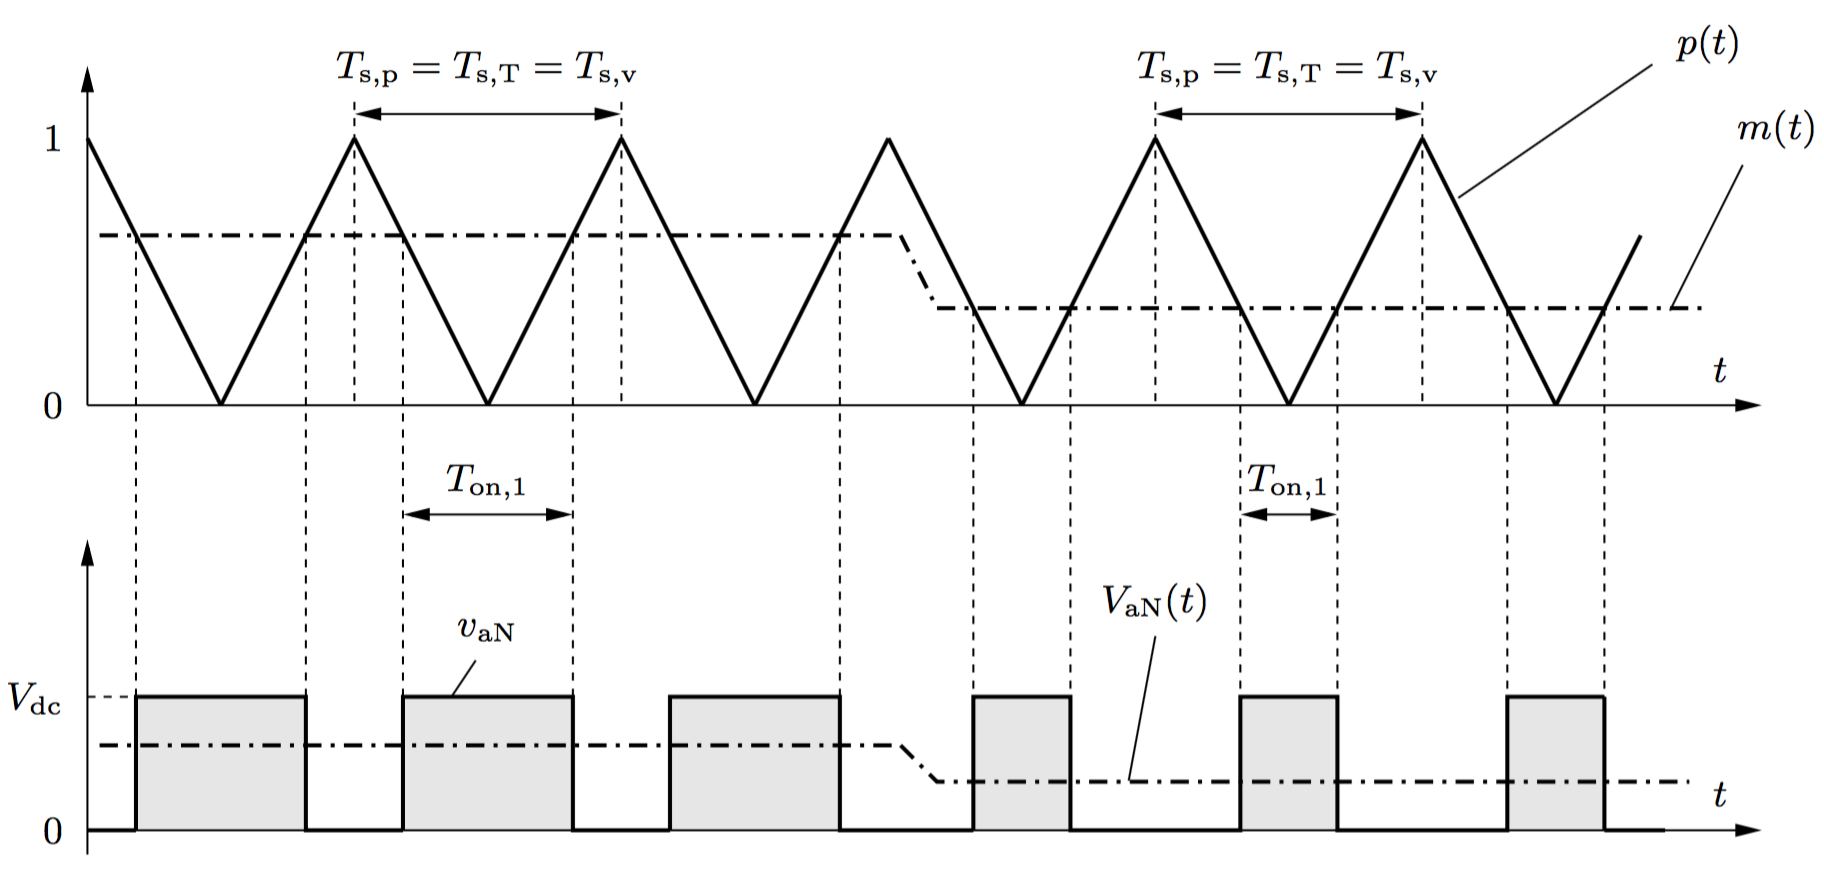
\includegraphics[scale=0.2]{ch4/6}
			\captionof{figure}{}
			\end{wrapfigure}
			Comme la tension de sortie $v_{aN}(t)$ est toujours positive ou nulle, on prend p(t) triangulaire variant entre 0 et 1. La m(t) est supposée varier lentement (constante sur une période de commutation $T_{s,p}$) par rapport à la porteuse. Quand $m(t) > p(t)$, l'interrupteur supérieur du bras est fermé et $v_{aN} = V_{dc}$. Quand $m(t) < p(t)$, c'est l'interrupteur inférieur qui est fermé et $v_{aN}$ = 0. On suppose que la m(t) est aussi comprise entre 0 et 1 de telle manière que p et m se croisent 2x par période de commutation $T_{s,p}$ et les interrupteurs s'ouvrent et se ferment à la même fréquence, qu'on retrouve aussi dans $v_{aN}$ : 
			\begin{equation}
				f_{s,p} = f_{s,T} = f_{s,v}. 
			\end{equation}
			Nous définissons le \textbf{rapport cyclique} (duty cycle) d'un interrupteur come la fraction du temps pendant laquelle il est fermé $0<D_x<1$. Pour T1 et T2 en négligeant le temps mort cela donne : 
			\begin{equation}
				D_1 = \frac{T_{on,1}}{T_s} \qquad et \qquad D_2 = \frac{T_{on,2}}{T_s} = \frac{T_s - T_{on,1}}{T_s} = 1 - D_1.
			\end{equation}
			Par convention, D d'un bras est celui de son interrupteur supérieur, donc $D = D_1$. Dans le cas présent :
			\begin{equation}
				D(t) = m(t). 
			\end{equation}
			On définit la \textbf{moyenne rapide} de $v_{aN}$ (moyennage sans harmoniques de commutation) : 
			\begin{equation}
				V_{aN}(t) = \frac{1}{T_s}\int _{t-T_s/2}^{t+T_s/2} v_{aN}(t') \, dt'
			\end{equation}
			qui varie lentement par rapport à $T_s$. On retrouve alors  approximativement : 
			\begin{equation}
				V_{aN}(t) = m(t) V_{dc}. 
			\end{equation}
			
		\subsubsection{Avec point milieu à l'entrée}
			Puisque $V_{aO}(t) = V_{aN}(t) - V_{dc}/2$ peut être positive ou négative, il peut fonctionner aussi bien en onduleur/redresseur qu'en hacheur. En prenant le même $p(t)$, on a toujours $D(t) = m(t)$ :
			\begin{equation}
				V_{aO}(t) = V_{aN}(t) - V_{dc}/2 = (m(t) - \frac{1}{2})V_{dc} \qquad et \qquad f_{s,p} = f_{s,T} =f_{s,v}
			\end{equation}
			
	\subsection{Pont en H}
		\subsubsection{Modulation bipolaire}
			Dans ce cas, on peut se limiter à un seul p(t) et m(t), en commandant les 4 interrupteurs de façon diagonale ($T^a$ avec $T_b$ et $T_a$ avec $T^b$). On n'utilise qu'une seule p(t) et un m(t) comme précédemment. Ainsi, $v_{ab}(t)$ vaut soit $V_{dc}$ soit $-V_{dc}$, pas de valeur nulle. On parle de \textbf{commutation bipolaire} du fait qu'il faille combiner les 2 valeurs de tension. La commutation diagonale implique $v_{bO}(t) = - v_{aO}(t)$ et la tension de sortie vaut le double de celle en demi-pont point milieu :
			\begin{equation}
				v_{ab}(t) = v_{aO}(t)-v_{bO}(t) = 2v_{aO}(t) \qquad \Rightarrow \qquad V_{ab}(t) = (2D(t)-1)V_{dc} = m(t) V_{dc},
			\end{equation}
			où D(t) est le rapport cyclique du premier bras. Les 3 $f_s$ sont toujours égales.
			
		\subsubsection{Modulation unipolaire}
			\begin{wrapfigure}[14]{l}{8cm}
			\vspace{-5mm}
			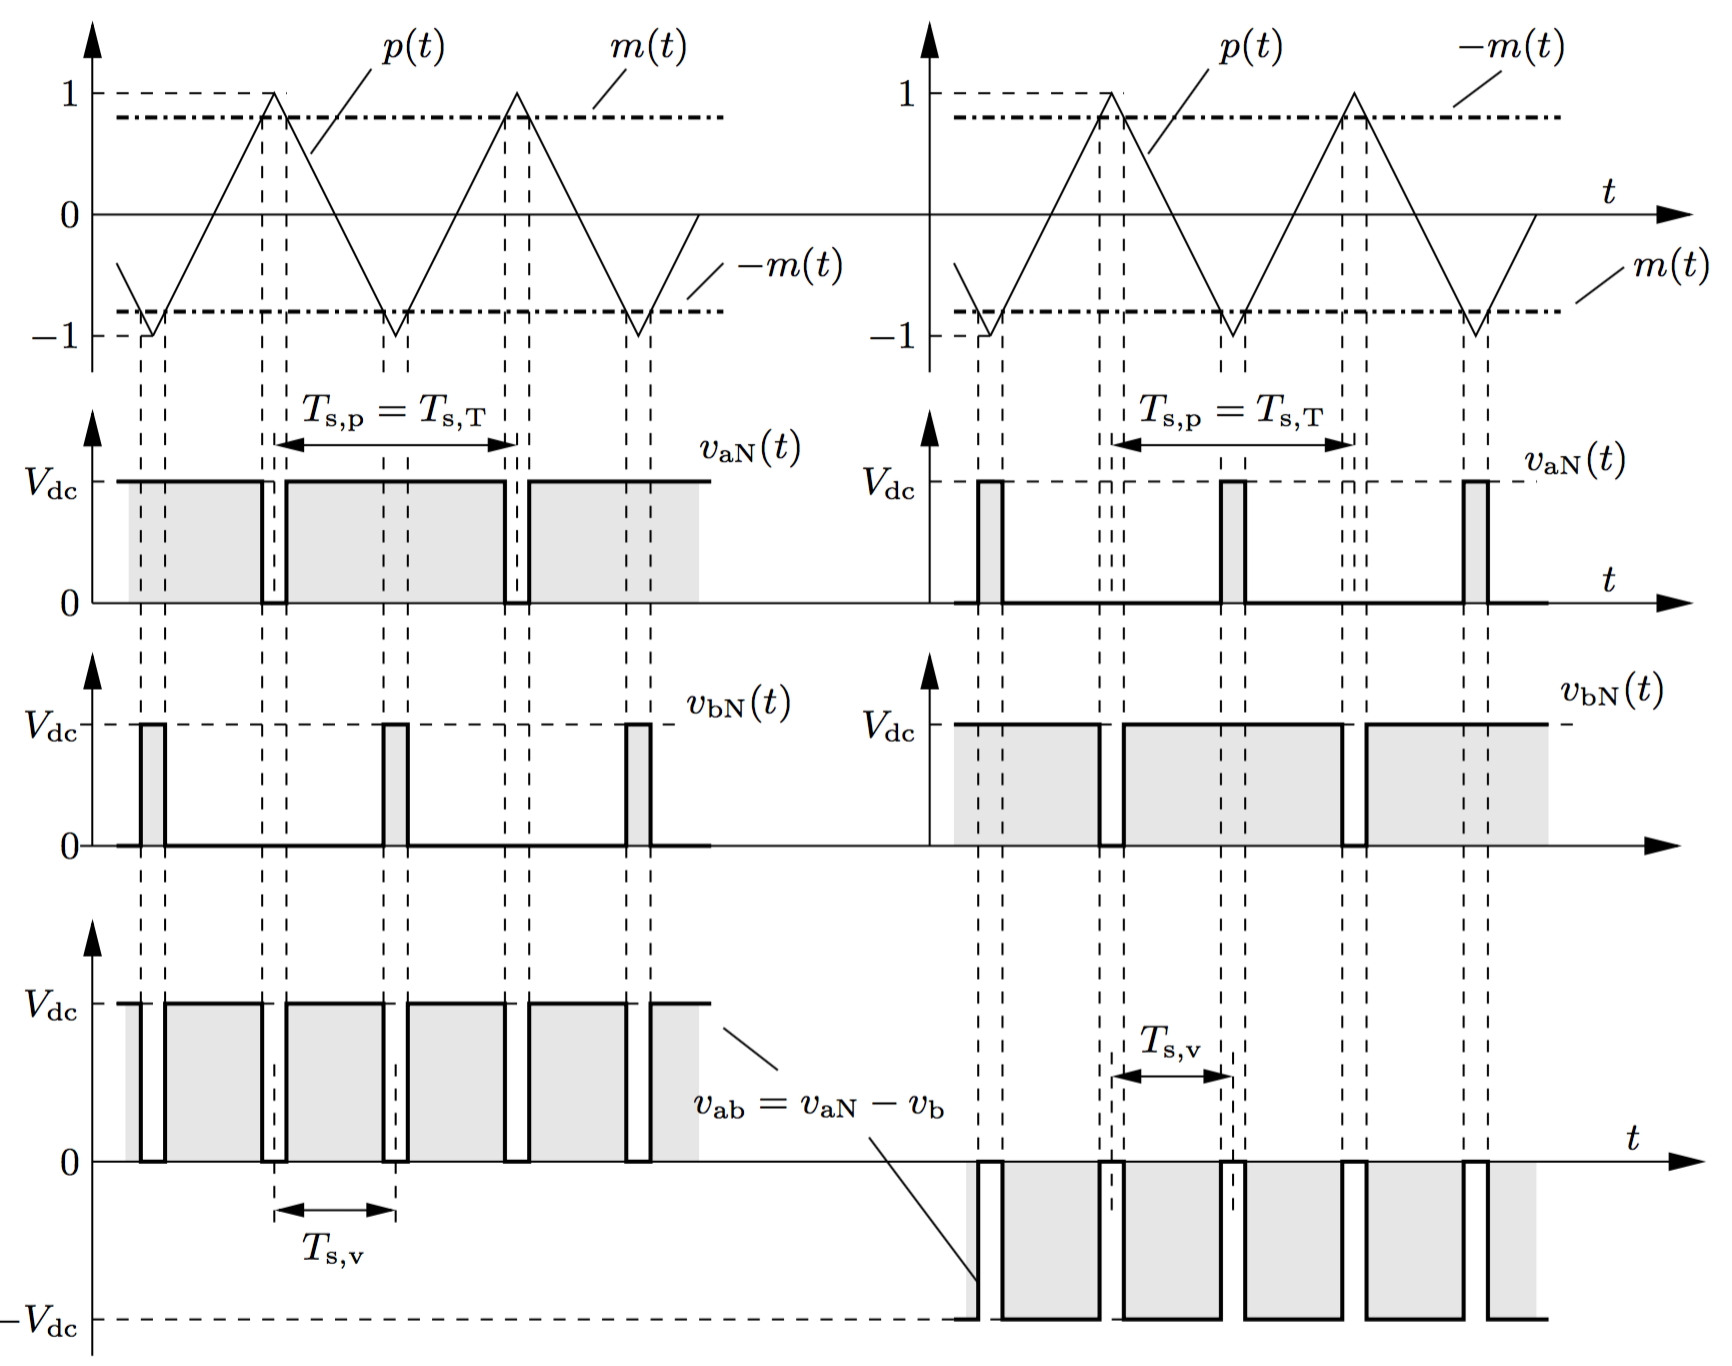
\includegraphics[scale=0.25]{ch4/11}
			\captionof{figure}{}
			\end{wrapfigure}
			On peut aussi utiliser 2 m(t) différentes pour les 2 bras. La p(t) varie maintenant entre -1 et 1, avec une m(t) pour la commande du premier bras et -m(t) pour celle du second. Lorsque $m(t) > 0$, $v_{ab}(t)$ comprend 2 impulsions positive entre 0 et $V_{dc}$ par période de commutation. Il vient alors :
			\begin{equation}
				2 f_{s,p} = 2f_{s,T} = f_{s,v}.
			\end{equation}
			Remarquons les intervalles à sortie nulle, court-circuit de la charge. La tension de sortie est pareil que le précédent cas. \\
			
		\subsubsection{Comparaison des schémas bipolaire et unipolaire}
			\begin{wrapfigure}[8]{r}{6.5cm}
			\vspace{-5mm}
			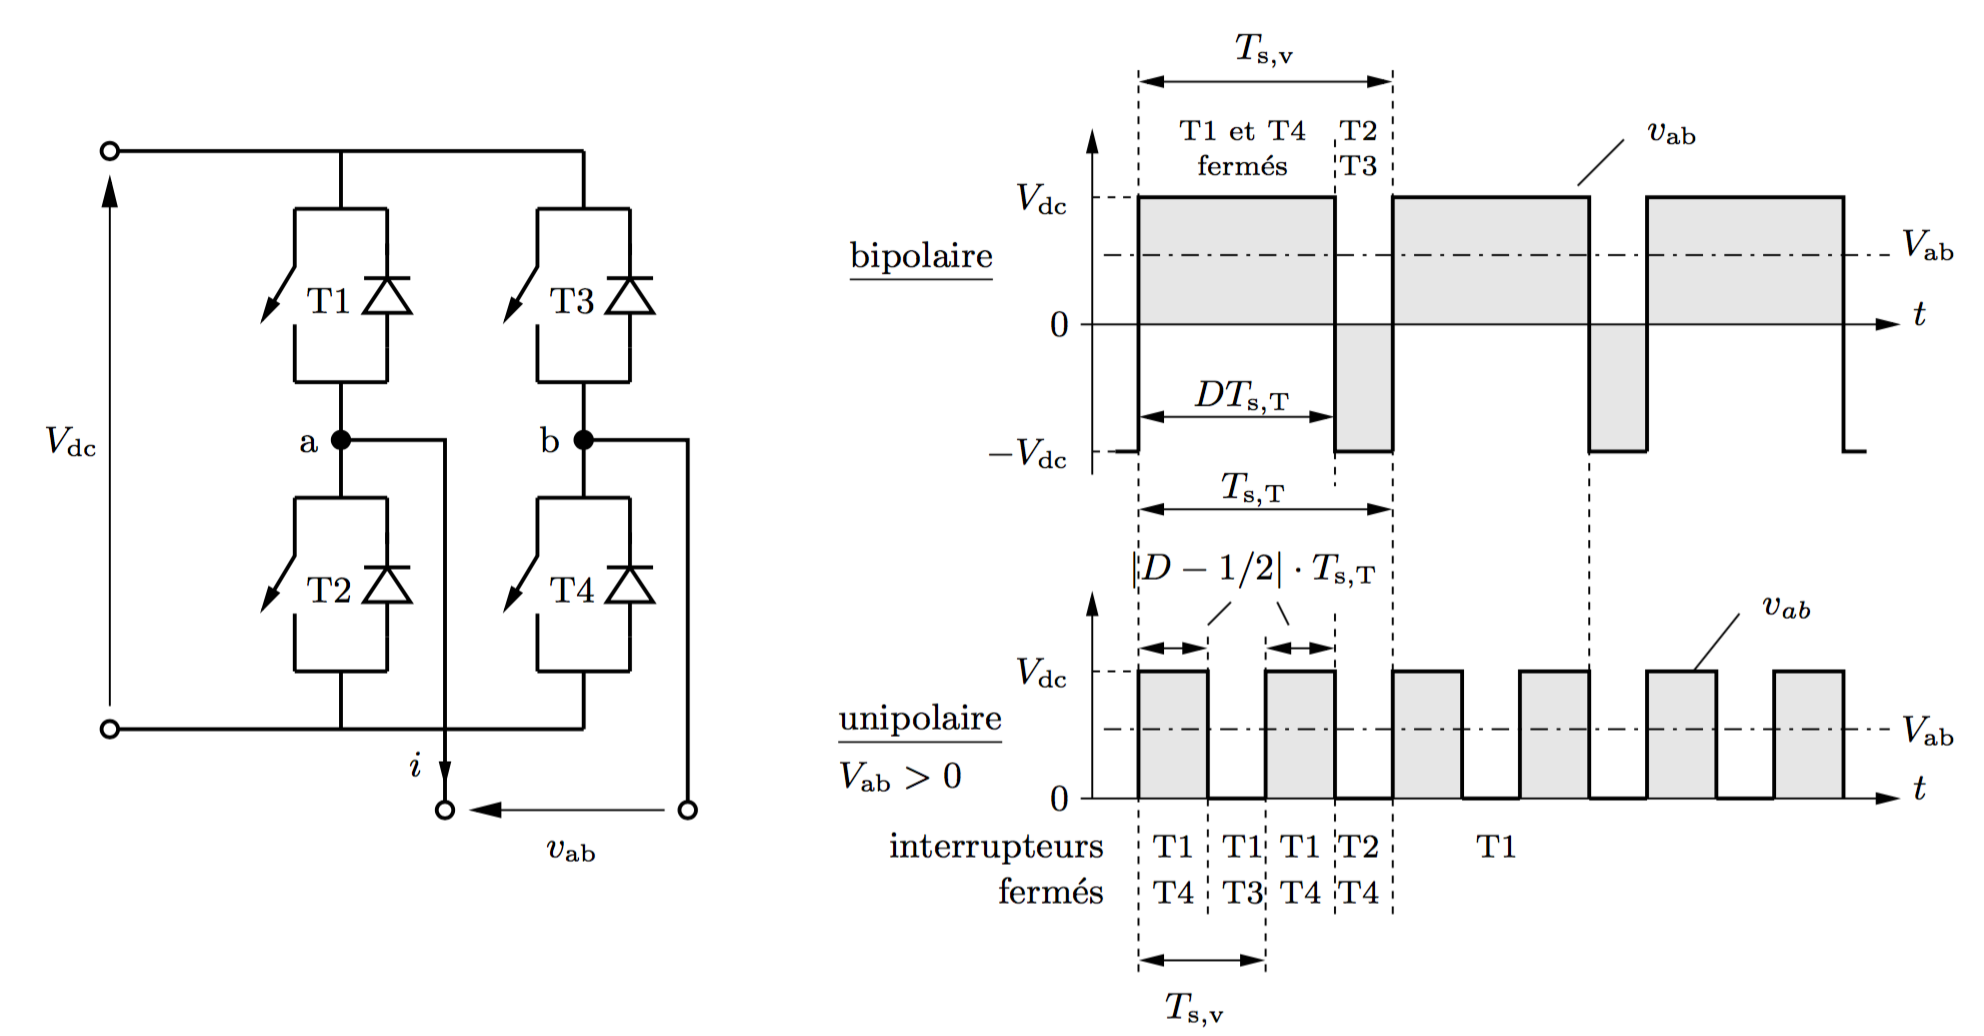
\includegraphics[scale=0.2]{ch4/12}
			\captionof{figure}{}
			\end{wrapfigure}
			Dans le cas bipolaire, on a par période de commutation, une impulsion positive de durée $DT_{s,T}$ et une impulsion négative de durée $(1-D)T_{s,T}$. Dans le cas unipolaire, par période de commutation on a 2 impulsions de même signe et de durée $|D-1/2|T_{s,T}$. L'écart entre les 2 cas est d'autant plus grand que D est proche de 0.5.
			\newpage
			
	\subsection{Couverture dans le plan tension-courant}
		\begin{wrapfigure}[10]{l}{7.5cm}
		\vspace{-5mm}
		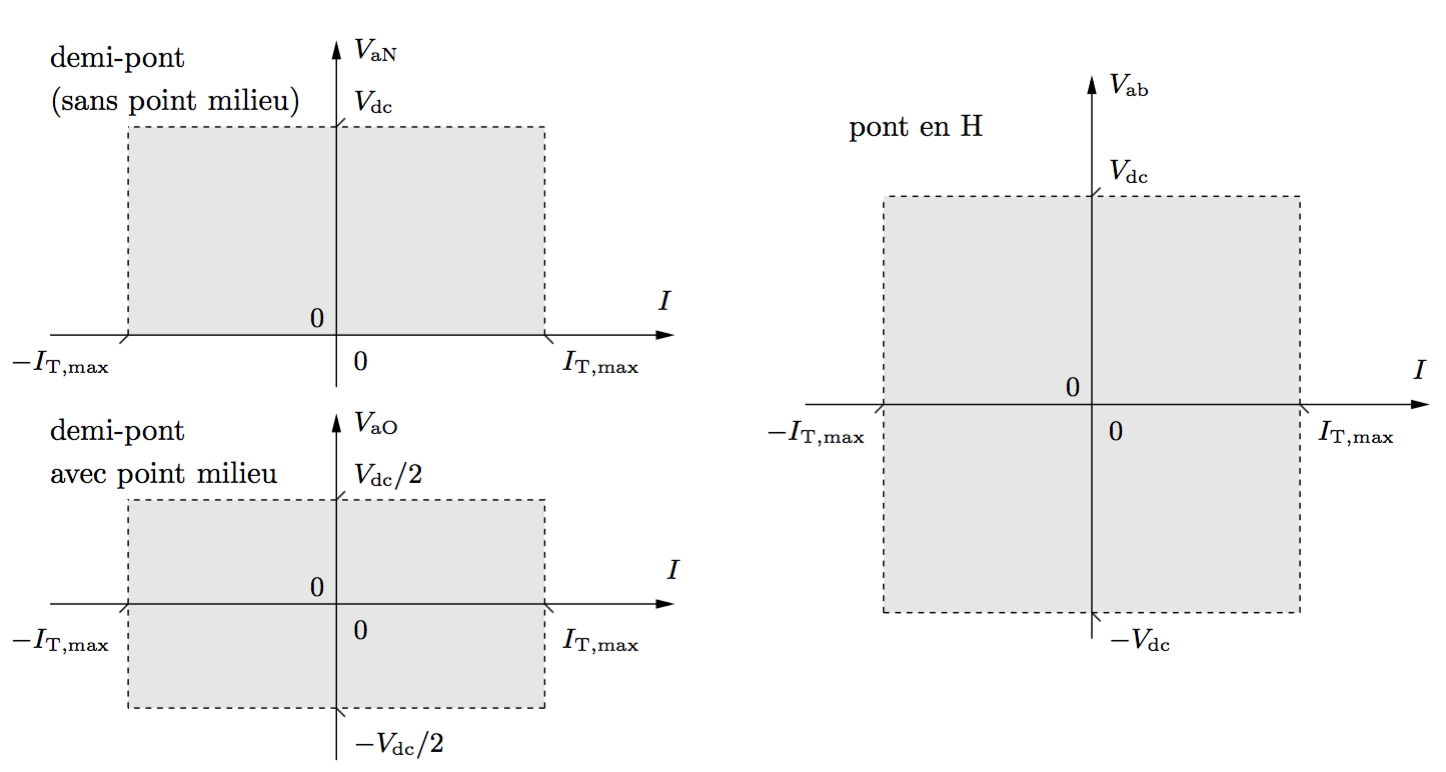
\includegraphics[scale=0.28]{ch4/13}
		\captionof{figure}{}
		\end{wrapfigure}
		Les \textbf{hacheurs} effectuent une conversion DC-DC entre $V_{dc}$ positive à l'entrée et une sortie moyenne positive ou négative $V_{aN}, V_{aO}$ ou $V_{ab}$. Pas de contrainte sur le signe de $i(t)$ mais sa valeur moyenne doit être limité : $-I_{T,min}\leq I \leq I_{T,max}$. En fonction du signe du courant par rapport à celle de la tension de sortie, la puissance s'écoule dans un sens. On distingue alors 4 quadrants dans le plan tension versus courant pour les hacheurs. 
		
	\subsection{Déformation du courant absorbé par une charge inductive}
		\begin{wrapfigure}[8]{r}{9cm}
		\vspace{-5mm}
		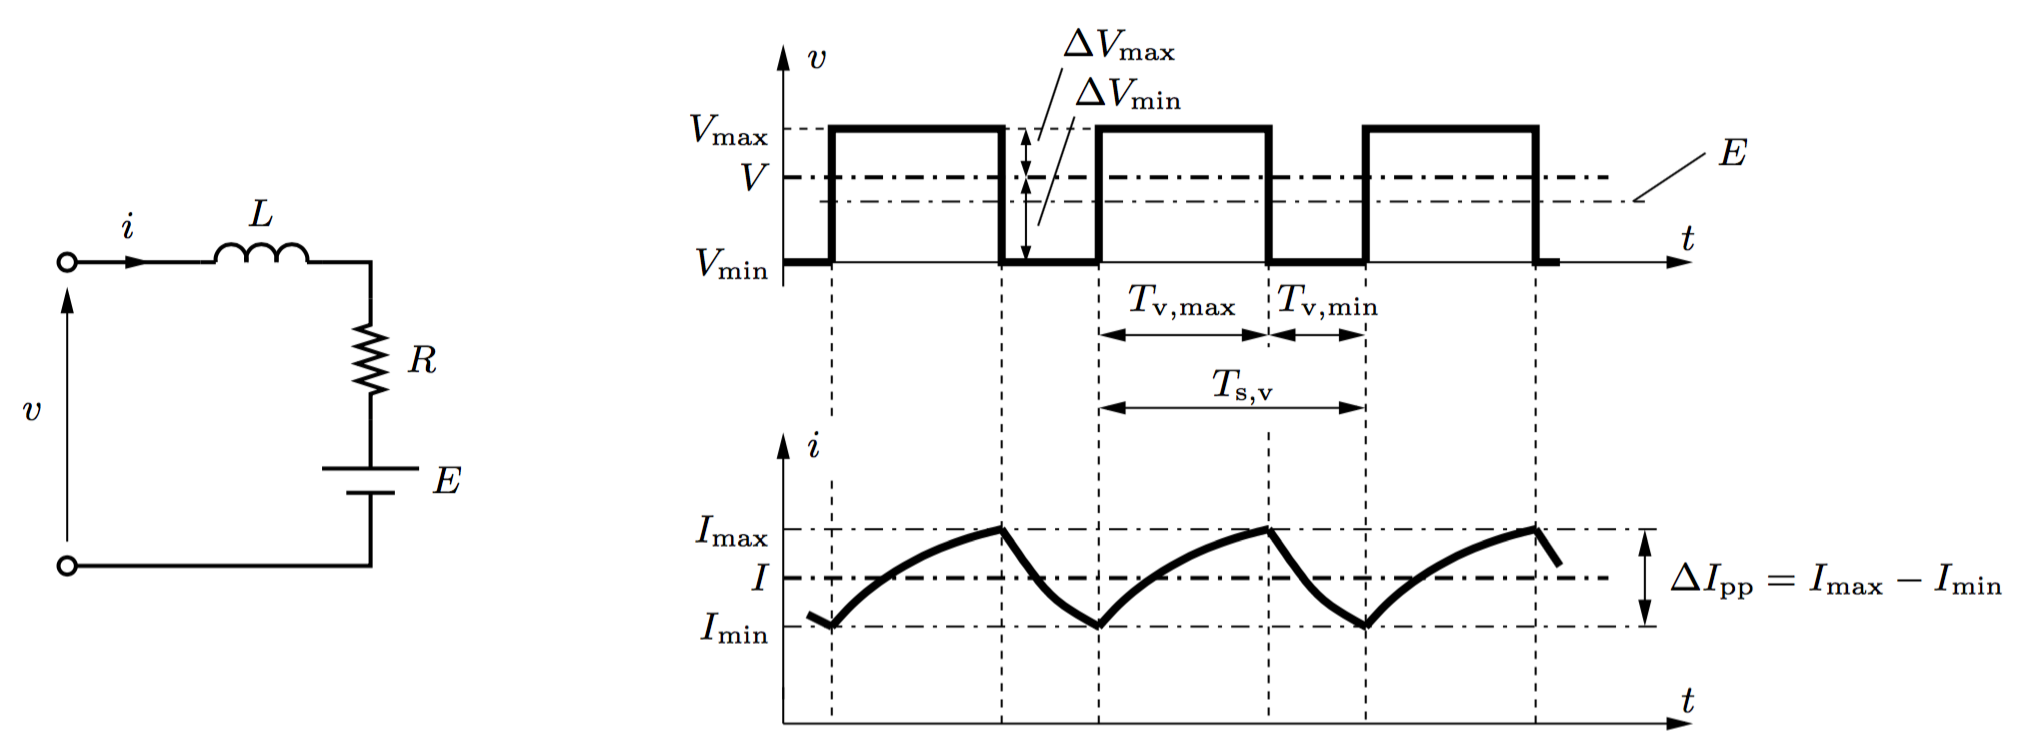
\includegraphics[scale=0.25]{ch4/14}
		\captionof{figure}{}
		\end{wrapfigure}
		Soit une charge RLE alimenté par une tension qui oscille entre $V_{min}$ et $V_{max}$, avec une période $T_{s,v}$ qui dépend de $f_{s,T}$ et du type de MLI. On considère le cas simplifié d'un régime établi et d'une tension $E=cst$. Les valeurs instantannées et moyennes sont relié comme suit :\\
		\begin{equation}
			v(t) = Ri(t) + L\frac{di}{dt} + E \qquad et \qquad V = RI + E.
		\end{equation}
		
		En soustrayant ces deux équations, on trouve pour les variations :
		\begin{equation}
			\Delta v(t) = R\delta i(t) + L\frac{d\Delta i}{dt}.
		\end{equation}
		$\Delta v(t)$ est constante par morceau et vaut $\Delta V_{max}$ pendant un intervalle $T_{v,max}$ et $\Delta V_{min}$ pendant $T_{v,min}$, avec $T_{v,min} + T_{v,max} = T_{s,v}$. Comme la valeur moyenne de $\Delta v(t) = 0$, on a :
		\begin{equation}
			\Delta V_{max}T_{v,max} + \Delta V_{min}T_{v,min} = 0 \qquad avec \qquad \Delta V_{max} \geq 0 \ et \ \Delta V_{min} \leq 0
		\end{equation}
		$i(t)$ varie en dents de scie avec des flancs montant de durée $T_{v,max}$ et descendant $T_{v,min}$. Si la constante de temps $\tau = L/R \gg T_{s,v}$, la pente des flancs peut être vu constant et vaut soit $\Delta V_{max}/L$ soit $\Delta V_{min}/L$. L'ondulation crête à crête de $\Delta i(t)$ et $i(t)$ est donnée par :
		\begin{equation}
			\Delta I_{pp} = \frac{\Delta V_{max}T_{v,max}}{L} = -\frac{\Delta V_{min}T_{v,min}}{L}.
		\end{equation}
		
		L'augmentation de $I_{rms}$ en raison de l'ondulation donne lieu à :
		\begin{equation}
		\begin{array}{c}
			I_{rms} = \sqrt{I^2+(\Delta I_{rms})^2} \qquad avec \\
			\Delta I_{rms} = (\Delta i)_{rms} = \sqrt{\frac{1}{T_{s,v}}\int _{t_0}^{t0+T_{s,v}}(\Delta i)^2\, dt} = \Delta I_{pp} \sqrt{\int _{-1/2}^{1/2}x^2\, dx} 
		\end{array}
		\end{equation}
		Il vient finalement que :
		\begin{equation}
			\Delta I_{rms} = \frac{1}{2\sqrt{3}}\Delta I_{pp}.
		\end{equation}
		Les pertes Joules supplémentaires dans R de la charge sont $R(\Delta I_{rms})^2$. \\
		
		\textbf{Demi-pont snas point milieu à l'entrée} \qquad On a $T_{s,v} = T_{s,T}$, $V_{aN} = DV_{dc}, T_{v,max} = DT_s, \Delta V_{max} = V_{dc}-V_{aN}= (1-D)V_{dc}$ et il vient que :
		\begin{equation}
			\Delta I_{pp} = (1-D)D\frac{V_{dc}}{f_{s,T}L}= (1-D)\frac{V_{aN}}{f_{s,T}L}. 
		\end{equation}
		On peut donc diminuer l'ondulation en augmentant L et/ou $f_{s,T}$. Elle dépend aussi de D et est maximum pour D = 0.5. \\
		
		\textbf{Demi-pont avec point milieu à l'entrée} \qquad On a $T_{s,v} =T_{s,T}, V_{aO} = (2D-1)V_{dc}/2, T_{v,max}=DT_{s,T}, \Delta V_{max} = V_{dc}/2-V_{aO = (1-D)V_{dc}}$ et il vient :
		\begin{equation}
			\Delta I_{pp} = (1-D)D\frac{V_{dc}}{f_{s,T}L} = \frac{2(1-D)D}{2D-1}\frac{V_{aO}}{f_{s,T}L}.
		\end{equation}
		\ \\
		
		\textbf{Pont en H et schéma bipolaire}\qquad On a $T_{s,v} = T_{s,T}, V_{ab}=(2D-1)V_{dc}, T_{v,max}=DT_{s,T}, \Delta V_{max}= V_{dc}-V_{ab}=2(1-D)V_{dc}$ et :
		\begin{equation}
			\Delta I_{pp} = 2(1-D)D\frac{V_{dc}}{f_{s,T}L} = \frac{2(1-D)D}{2D-1}\frac{V_{ab}}{f_{s,T}L}.
		\end{equation}
		
		\ \\ \textbf{Pont en H et schéma unipolaire} \qquad On a en considérant une tension moyenne positive ($0.5\leq D\leq 1$) $T_{s,v} = T_{s,T}/2, V_{ab} =(2D-1)V_{dc}\geq 0, V_{max}=V_{dc}, T_{v,max}=(D-0.5)T_{s,T}, V_{min}=0, T_{v,min}= (1-D)T_{s,T}, \Delta V_{max}= V_{dc}-V_{ab}=2(1-D)V_{dc}$ et :
		\begin{equation}
			\Delta I_{pp} = (1-D)(2D-1)\frac{V_{dc}}{f_{s,T}L} = (1-D)\frac{V_{ab}}{f_{s,T}L}
		\end{equation}
		
		Pour une tension moyenne négative ($0\leq D\leq 0.5$) $T_{s,v} = T_{s,T}/2, V_{ab} =(2D-1)V_{dc}\leq 0, V_{max}=0, T_{v,max}=DT_{s,T}, V_{min}=-V_{dc}, T_{v,min}= (0.5-D)T_{s,T}, \Delta V_{max}= 0-V_{ab}=(1-2D)V_{dc}$ et :
		\begin{equation}
			\Delta I_{pp} = D(1-2D)\frac{V_{dc}}{f_{s,T}L} = D\frac{-V_{ab}}{f_{s,T}L}.
		\end{equation}
		Le schéma unipolaire donne lieu à un courant beaucoup moins ondulé que le cas bipolaire quand on s'éloigne des cas extrême D = 0 ou D=1. La différence est la plus grande quand D=0.5. Ces expressions restent valables dans le transitoire à condition de pouvoir scinder la variation fondamentale des grandeurs et celle qui est due aux commutations.
		
	\subsection{Temps mort}
		\begin{wrapfigure}[11]{l}{7cm}
		\vspace{-5mm}
		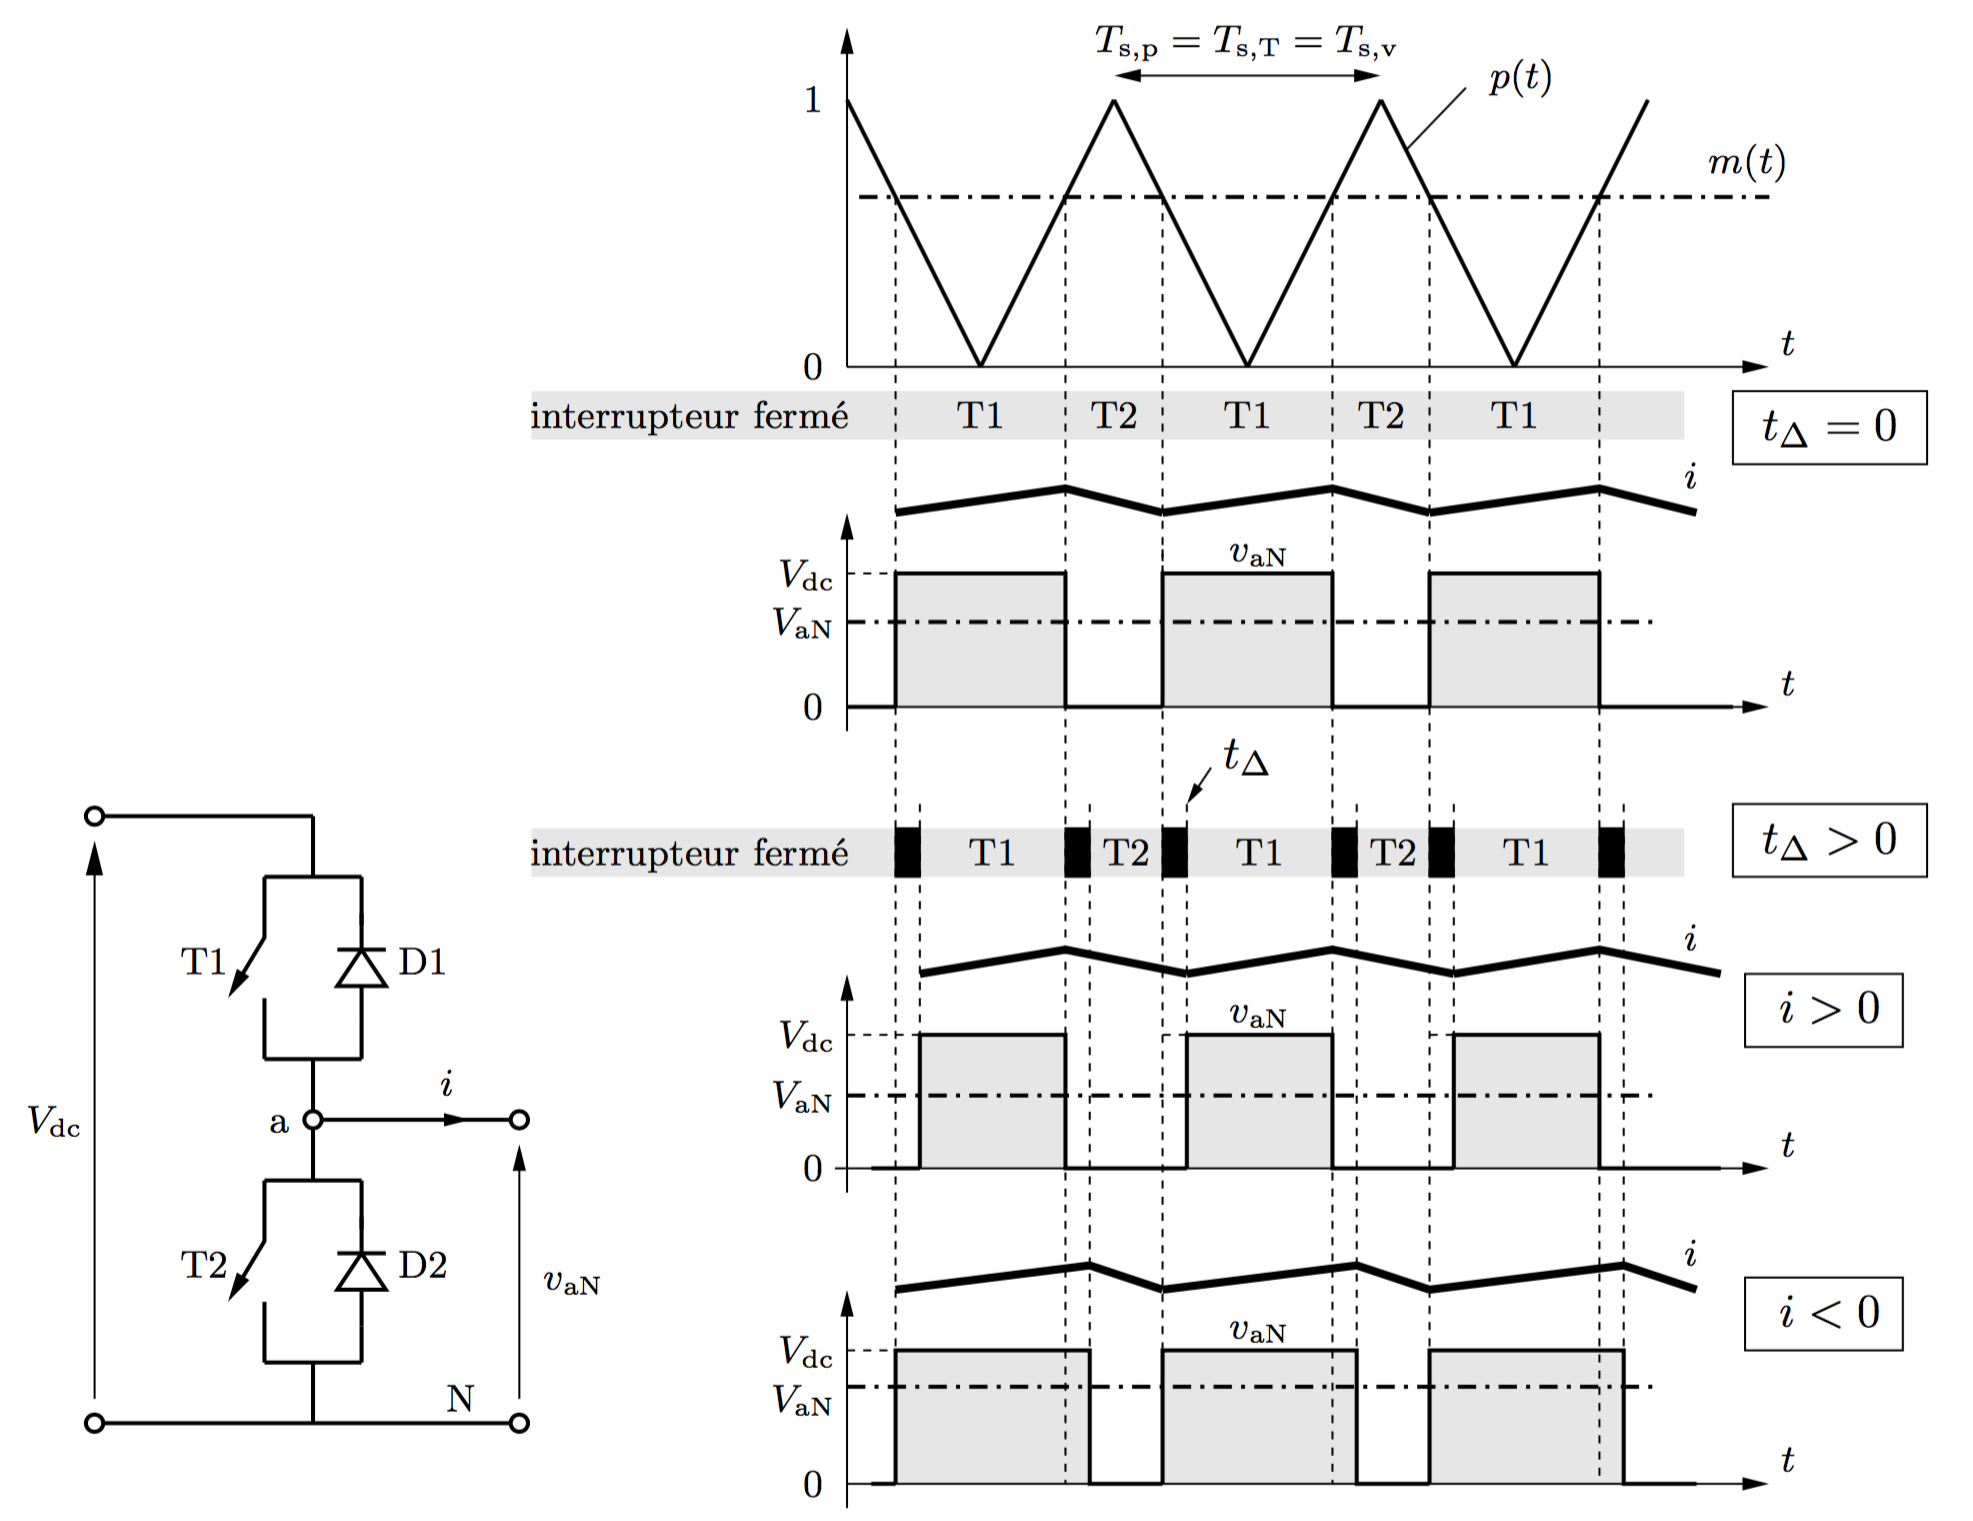
\includegraphics[scale=0.2]{ch4/15}
		\captionof{figure}{}
		\end{wrapfigure}
		Il faut dans la pratique intercaller un court intervalle durant lequel les 2 interrupteurs d'un bras sont ouverts pour éviter un court-circuit lors des commutations. Dans le cas d'un \textbf{demi-pont}, durant les courts instants où T1 et T2 sont ouverts en même temps, le sens de $i$ détermine la valeur de $v_{aN}$. S'il est >0, il circulera dans D2 et $v_{aN} =0$, si $i<0$, il circulera dans D1 et $v_{aN} = V_{dc}$. La figure ci-contre montre l'effet d'un report de la \textbf{fermeture} sur la tension de sortie, en supposant une charge inductive pour que $i$ faiblement ondulé ne s'inverse pas. 
		
\section{Onduleurs de tension monophasés}
	\begin{wrapfigure}[10]{l}{10cm}
	\vspace{-5mm}
	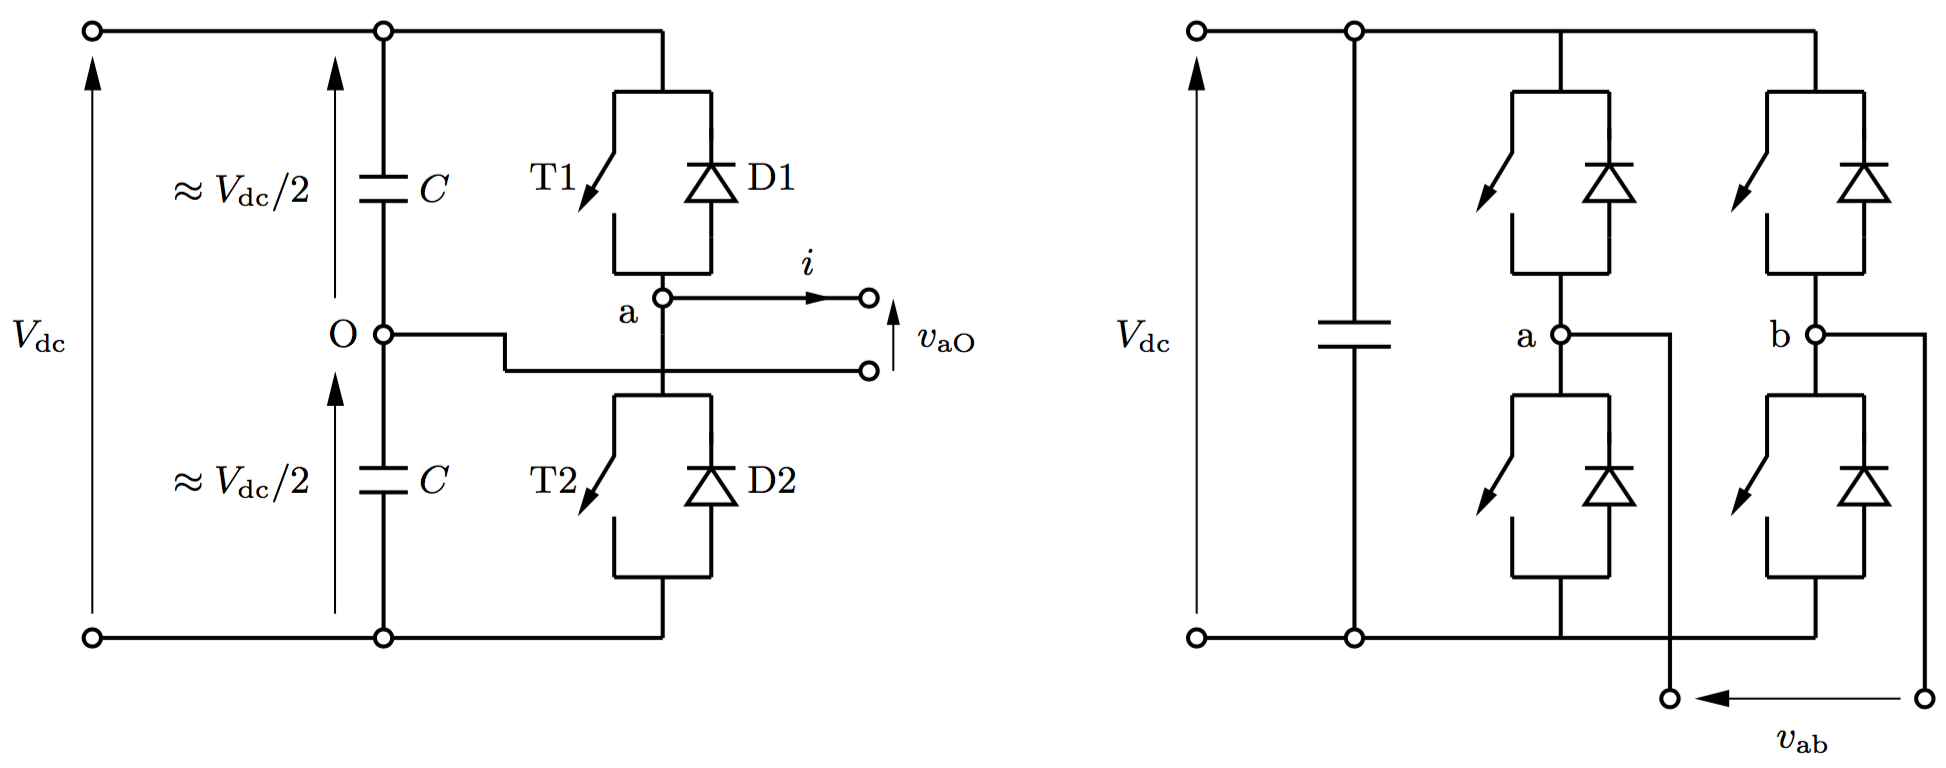
\includegraphics[scale=0.28]{ch4/16}
	\captionof{figure}{}
	\end{wrapfigure}
	Ils sont constitués d'1 ou 2 bras. Un demi-pont doit être muni d'un point milieu à la source. Au besoin on crée le crée à l'aide de 2 condensateurs de même C élevée.  Pour le pont en H c'est pas nécessaire. Dans la pratique, l'onduleur est alimenté par un redresseur, d'où le lissage par condensateur à l'entrée. Si la source est une batterie, le condensateur prend en charge la composante ondulatoire du courant et atténue l'effet de la résistance interne pendant que la batterie fournit la composante moyenne. 
	
	\subsection{MLI sinusoïdale linéaire}
		\subsubsection{Demi-pont}
			\begin{wrapfigure}[14]{r}{7cm}
			\vspace{-5mm}
			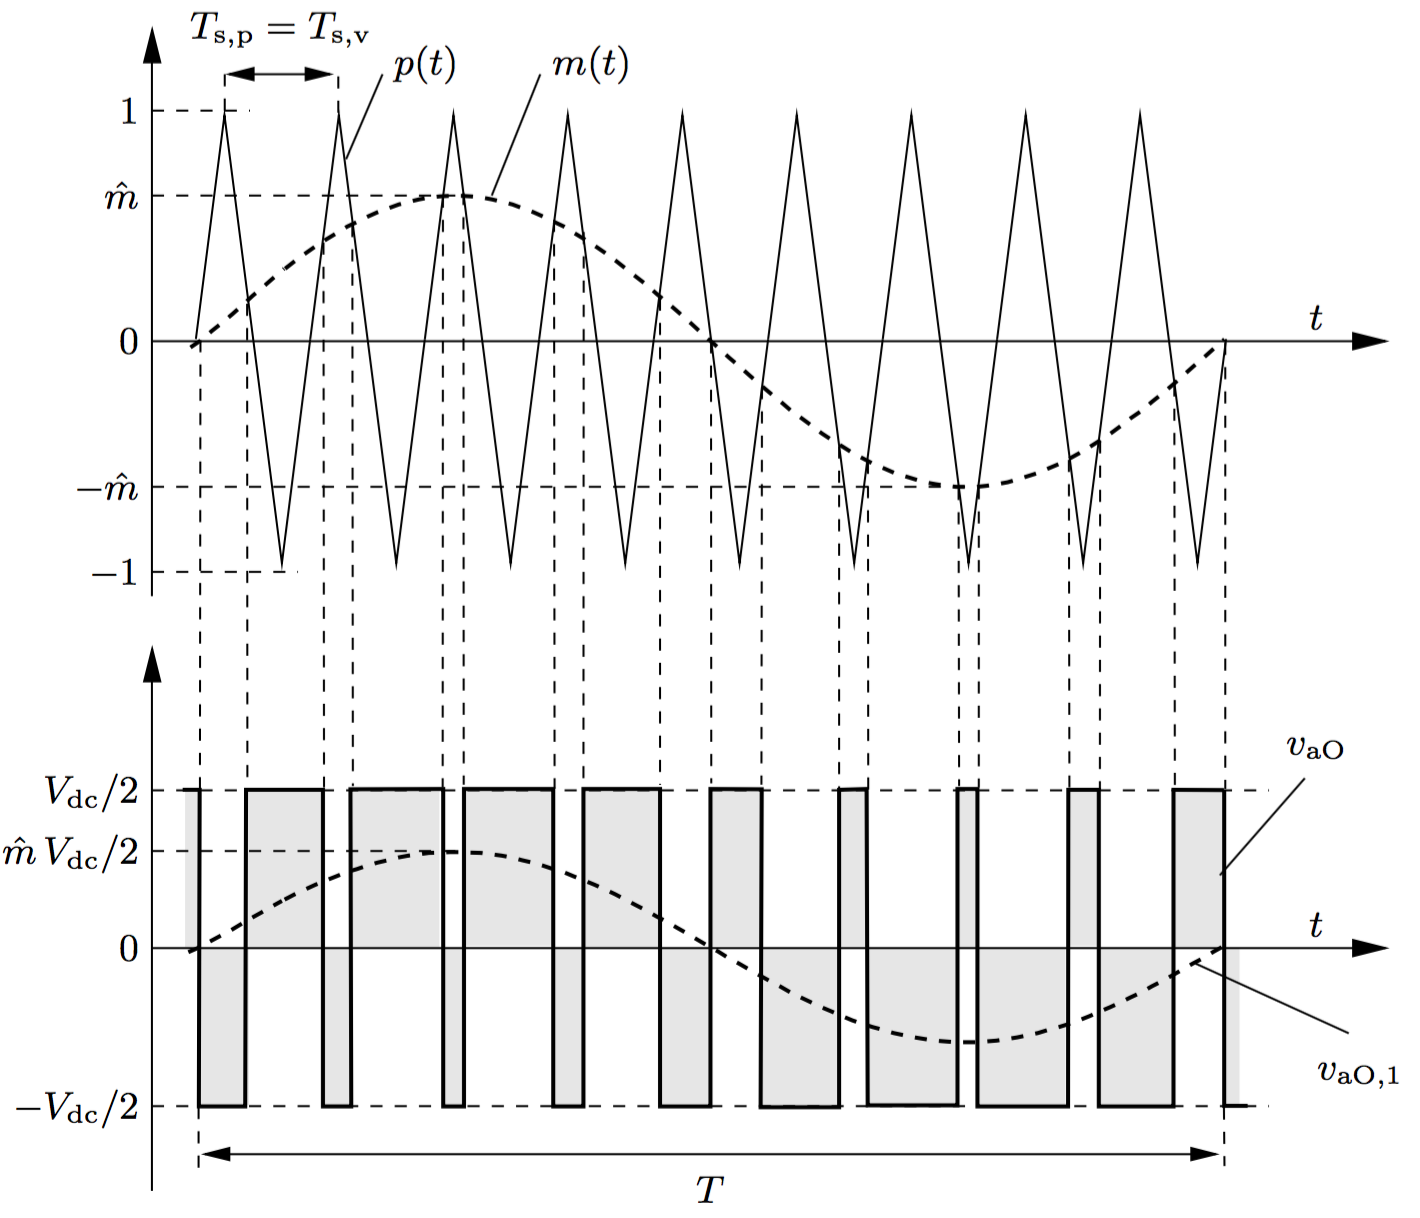
\includegraphics[scale=0.28]{ch4/17}
			\captionof{figure}{}
			\end{wrapfigure}
			On prend pour $p(t)$ un signal triangulaire de fréquence $f_{s,p}$ variant entre -1 et 1 et pour $m(t)$ une sinusoïde de fréquence $f$ et amplitude $\hat{m}$, image de la tension souhaitée. L'\textbf{angle de phase} constitue le 3ème degré de liberté pour $m(t)$. On définit l'\textbf{indice d'amplitude} qui est le rapport des valeurs crêtes :
			\begin{equation}
				\hat{m} = \frac{\hat{m}}{1}
			\end{equation}
			Nous supposons dans un premier temps qu'il est $<1$. On définit également l'\textbf{indice de fréquence} : 
			\begin{equation}
				m_f = \frac{f_{s,p}}{f}.
			\end{equation}
			Il est de préférence \textbf{entier} (MLI synchrone) et dans le cas du demi-pont, impair). Avec $m_f$ entier et impair, $v_{aO}(t)$ possède la symétrie demi-onde $v_{aO}(t) = - v_{aO}(t+T/2)$, faisant disparaître les harmoniques paires. Lorsque $\hat{m}\leq 1$, m(t) et p(t) se croisent 2 fois par période de commutation $T_{s,T} = T_{s,p}$.\\
			
			 Si $m_f$ est suffisamment grand ($\geq 9$ par ex.) m(t) varie lentement comparé à p(t) et les discussions sur les hacheurs sont d'application. Il vient alors pour l'amplitude de la findamentale $\hat{V}_{aO,1}$ : 
			 \begin{equation}
			 	\hat{V}_{aO,1} = \hat{m}\frac{V_{dc}}{2}.
			 \end{equation}
			 On parle alors de \textbf{modulation linéaire}. Outre la composante fondamentale de fréquence f, la tension comprend des harmoniques de fréquences élevée (pas de faible !) dont le rang impair s'écrit $h = km_f \pm l$ avec $k=1,2,...$ et $l$ entier et petit. 
			
		\subsubsection{Pont en H}
			
				